
\section{Highest Roll EV}

\begin{exerciseBox}[Highest Roll EV]
Jim will roll a fair, six-sided die until he gets a 4. \\
\textbf{Question :}  What is the expected value of the highest number he rolls through this process ?
\end{exerciseBox}


\subsection*{Solution :}

On note $T=\inf\{n\ge 1:\ X_n=4\}$ le rang d'apparition du premier $4$, et
\[
M=\max\{X_1,\dots,X_T\}
\]
le maximum observé jusqu'à (et incluant) ce premier $4$.

Comme le processus s'arrête dès l'apparition de $4$, on a nécessairement
\[
M\in\{4,5,6\}.
\]
On calcule alors $\mathbb{P}(M=4)$, $\mathbb{P}(M=5)$ et $\mathbb{P}(M=6)$.

\medskip
\noindent\textbf{1. Calcul de $\mathbb{P}(M=4)$.}\\
L'événement $\{M=4\}$ signifie : \emph{aucun $5$ ni $6$ n'apparaît avant le premier $4$}.
Autrement dit, le premier élément de $\{4,5,6\}$ observé est $4$.
Ainsi,
\[
\mathbb{P}(M=4)=\mathbb{P}(T_4< T_{\{5,6\}})
=\frac{\mathbb{P}(X_1=4)}{\mathbb{P}(X_1=4)+\mathbb{P}(X_1\in\{5,6\})}
=\frac{\frac16}{\frac16+\frac26}
=\frac13.
\]

\medskip
\noindent\textbf{2. Calcul de $\mathbb{P}(M\le 5)$ et $\mathbb{P}(M=6)$.}\\
On a $\{M\le 5\}$ si et seulement si \emph{aucun $6$ n'apparaît avant le premier $4$}, c'est-à-dire
le premier élément de $\{4,6\}$ observé est $4$ :
\[
\mathbb{P}(M\le 5)=\mathbb{P}(T_4<T_6)
=\frac{\mathbb{P}(X_1=4)}{\mathbb{P}(X_1=4)+\mathbb{P}(X_1=6)}
=\frac{\frac16}{\frac16+\frac16}
=\frac12.
\]
Par complément,
\[
\mathbb{P}(M=6)=1-\mathbb{P}(M\le 5)=\frac12.
\]

\medskip
\noindent\textbf{3. Calcul de $\mathbb{P}(M=5)$.}\\
On en déduit
\[
\mathbb{P}(M=5)=\mathbb{P}(M\le 5)-\mathbb{P}(M=4)
=\frac12-\frac13
=\frac16.
\]

\medskip
\noindent\textbf{4. Espérance de $M$.}\\
Finalement,
\[
\mathbb{E}[M]
=4\,\mathbb{P}(M=4)+5\,\mathbb{P}(M=5)+6\,\mathbb{P}(M=6)
=4\cdot\frac13+5\cdot\frac16+6\cdot\frac12
=\frac{31}{6}.
\]
Ainsi,
\[
\boxed{\mathbb{E}[M]=\frac{31}{6}.}
\]



\section{Ten Floor Building}

\begin{exerciseBox}[Ten Floor Building]
Un immeuble possède $10$ étages au-dessus du sous-sol (étages $1,2,\dots,10$).
Au sous-sol, $12$ personnes montent dans un ascenseur. Chacune choisit indépendamment et
uniformément au hasard un étage parmi $\{1,\dots,10\}$ pour descendre.

Combien d'étages l'ascenseur s'arrêtera-t-il en moyenne (c'est-à-dire à combien d'étages
différents au moins une personne descendra) ?
\end{exerciseBox}

\subsection*{Solution :}

Pour chaque étage $i\in\{1,\dots,10\}$, on définit la variable indicatrice
\[
I_i=\mathbf{1}_{\{\text{l'ascenseur s'arrête à l'étage } i\}}.
\]
Alors le nombre total d'arrêts est
\[
S=\sum_{i=1}^{10} I_i,
\qquad\text{donc}\qquad
\mathbb{E}[S]=\sum_{i=1}^{10}\mathbb{E}[I_i]
\]
(par linéarité de l'espérance).

Or $\mathbb{E}[I_i]=\mathbb{P}(I_i=1)$ est la probabilité qu'au moins une des 12 personnes choisisse
l'étage $i$. Par complément :
\[
\mathbb{P}(I_i=1)=1-\mathbb{P}(\text{personne ne choisit } i)
=1-\left(\frac{9}{10}\right)^{12},
\]
car une personne évite l'étage $i$ avec probabilité $9/10$, et les choix sont indépendants.

Ainsi, pour tout $i$,
\[
\mathbb{E}[I_i]=1-\left(\frac{9}{10}\right)^{12}.
\]
Finalement,
\[
\boxed{
\mathbb{E}[S]
=
\sum_{i=1}^{10}\left(1-\left(\frac{9}{10}\right)^{12}\right)
=
10\left(1-\left(\frac{9}{10}\right)^{12}\right).
}
\]

\section{Temps d'attente (loi géométrique)}


\begin{exerciseBox}[Temps d'attente (loi géométrique)]
On répète une expérience aléatoire de manière indépendante et identiquement distribuée (i.i.d.).
À chaque essai, l'événement $A$ se produit avec probabilité $p=\mathbb{P}(A)$, avec $0<p\le 1$.
On définit le temps d'attente
\[
T=\inf\{n\ge 1:\ \text{$A$ se produit au $n$-ième essai}\}.
\]

\begin{enumerate}
\item \textbf{(Question générale)} Montrer que $T$ suit une loi géométrique et calculer
\[
\mathbb{P}(T=n)\quad (n\ge 1)
\qquad\text{et}\qquad
\mathbb{E}[T].
\]


\item \textbf{(Application : lancer de dé)}  
% On lance un dé équilibré de manière répétée jusqu’à obtenir la face $4$.
Combien de lancers doit-on effectuer \emph{en moyenne} pour obtenir pour la première fois la face $4$ ?

\end{enumerate}
\end{exerciseBox}


\subsection*{Solution :}


\begin{enumerate}
\item Pour que $T=n$, il faut que les $n-1$ premiers essais soient des échecs ($A^c$),
puis que le $n$-ième essai soit un succès ($A$). Par indépendance,
\[
\mathbb{P}(T=n)=\mathbb{P}(A^c)^{n-1}\mathbb{P}(A)=(1-p)^{n-1}p,\qquad n\ge 1.
\]
Ainsi $T$ suit une loi géométrique de paramètre $p$. De plus,
\[
\mathbb{E}[T]=\sum_{n=1}^{\infty} n\,\mathbb{P}(T=n)
=\sum_{n=1}^{\infty} n(1-p)^{n-1}p.
\]
Or on sait que, pour $|q|<1$,
\[
\sum_{n=1}^{\infty} n q^{n-1}=\frac{1}{(1-q)^2}.
\]
En prenant $q=1-p$ (avec $0\le q<1$), on obtient
\[
\mathbb{E}[T]=p\cdot \frac{1}{(1-(1-p))^2}=p\cdot \frac{1}{p^2}=\frac{1}{p}.
\]

\item Ici, $A=\{X=4\}$ pour un dé équilibré, donc $p=\mathbb{P}(A)=1/6$.
Par conséquent,
\[
nb_{moyenne} = \mathbb{E}[T]=\frac{1}{p}=6.
\]
\end{enumerate}


\section{Conditional Die Rolls 1}

\begin{exerciseBox}[Conditional Die Rolls]
Dan rolls a dice until he gets a 6. Given that he did not see a  5
, what is the expected number of times Dan rolled his die?


\end{exerciseBox}

\subsection*{Solution :}

On note $T$ le nombre de lancers nécessaires pour obtenir pour la première fois un $6$.

On considère l’événement
\[
E=\{\text{aucune face $5$ n’apparaît avant le premier $6$}\}.
\]

the expected number of times Dan rolled his die is : 
\[
\mathbb{E}[T\mid E] \, ?
\]

Pour $n\ge 1$, l’événement $\{T=n\}\cap E$ se réalise si et seulement si :
\begin{itemize}
\item les $n-1$ premiers lancers prennent des valeurs dans $\{1,2,3,4\}$,
\item le $n$-ième lancer est égal à $6$.
\end{itemize}
Ainsi,
\[
\mathbb{P}(T=n\cap E)
=
\left(\frac{4}{6}\right)^{n-1}\frac{1}{6}.
\]

On calcule ensuite la probabilité de $E$ :
\[
\mathbb{P}(E)
=
\sum_{n=1}^{\infty}\mathbb{P}(T=n\cap E)
=
\sum_{n=1}^{\infty}\left(\frac{4}{6}\right)^{n-1}\frac{1}{6}
=
\frac{\frac{1}{6}}{1-\frac{4}{6}}
=
\frac12.
\]

La loi conditionnelle de $T$ sachant $E$ est donc donnée par
\[
\mathbb{P}(T=n\mid E)
=
\frac{\mathbb{P}(T=n\cap E)}{\mathbb{P}(E)}
=
\left(\frac{2}{3}\right)^{n-1}\frac{1}{3},
\qquad n\ge 1.
\]
Il s'agit d'une loi géométrique de paramètre $p=\frac13$.
Par conséquent,
\[
\boxed{\mathbb{E}[T\mid E]=\frac{1}{p}=3.}
\]

\section{Conditional Die Rolls 2}


\begin{exerciseBox}[Conditional Die Rolls 2]
Dan lance un dé équilibré à six faces jusqu’à l’apparition du premier $6$.
Sachant qu’il a observé au moins un $5$ avant l’apparition du premier $6$,
déterminer l’espérance du nombre total de lancers effectués.
\end{exerciseBox}

\subsection*{Solution :}

On modélise l’expérience probabiliste de la manière suivante.

Soit $(X_n)_{n\geq 1}$ une suite de variables aléatoires indépendantes et identiquement distribuées,
où $X_n$ représente le résultat du $n$-ième lancer, avec
\[
\mathbb{P}(X_n = k) = \frac{1}{6}, \quad k=1,\dots,6.
\]

On définit la variable aléatoire
\[
N = \inf\{n \geq 1 \mid X_n = 6\},
\]
qui représente le nombre total de lancers nécessaires pour obtenir le premier $6$.

On conditionne par l’événement
\[
A = \{\text{au moins un } 5 \text{ apparaît avant le premier } 6\}.
\]

\medskip

\textbf{Étape 1 : temps d’apparition du premier $5$ ou $6$.}

Soit
\[
T = \inf\{n \geq 1 \mid X_n \in \{5,6\}\}.
\]
À chaque lancer,
\[
\mathbb{P}(X_n \in \{5,6\}) = \frac{2}{6} = \frac{1}{3}.
\]
Ainsi, $T$ suit une loi géométrique de paramètre $\frac{1}{3}$, et
\[
\mathbb{E}[T] = \frac{1}{1/3} = 3.
\]

Sous l’événement $A$, le premier élément de $\{5,6\}$ observé est nécessairement un $5$.

\medskip

\textbf{Étape 2 : temps d’attente du premier $6$ après un $5$.}

Après l’apparition du premier $5$, le processus recommence indépendamment.
Soit $M$ le nombre de lancers nécessaires pour obtenir un $6$ à partir de ce moment-là.
Alors $M$ suit une loi géométrique de paramètre $\frac{1}{6}$, et
\[
\mathbb{E}[M] = \frac{1}{1/6} = 6.
\]

\medskip

\textbf{Étape 3 : calcul de l’espérance conditionnelle.}

Sous l’événement $A$, le nombre total de lancers s’écrit
\[
N = T + M.
\]
Par linéarité de l’espérance,
\[
\mathbb{E}[N \mid A] = \mathbb{E}[T] + \mathbb{E}[M] = 3 + 6 = 9.
\]

\medskip

\[
\boxed{\mathbb{E}[N \mid \text{au moins un } 5 \text{ avant le premier } 6] = 9}
\]

\section{Conditional Die Rolls 3}

\begin{exerciseBox}[Conditional Die Rolls 3]
Dan lance un dé équilibré à six faces jusqu’à obtenir un $6$.
Sachant qu’il n’a observé que des nombres pairs pendant toute l’expérience,
quel est le nombre moyen  de lancers effectués ?
\end{exerciseBox}

\subsection*{Solution :}

On modélise les lancers par une suite $(X_n)_{n\ge 1}$ de variables aléatoires i.i.d. uniformes sur
$\{1,2,3,4,5,6\}$, c’est-à-dire
\[
\mathbb{P}(X_n=k)=\frac{1}{6},\qquad k\in\{1,2,3,4,5,6\}.
\]
On note
\[
N=\inf\{n\ge 1:\; X_n=6\}
\]
le nombre total de lancers jusqu’au premier $6$.

On conditionne par l’événement
\[
E=\{\text{tous les résultats observés (jusqu’à l’arrêt inclus) sont pairs}\}.
\]
Sur $E$, tous les lancers avant l’arrêt doivent appartenir à $\{2,4\}$, et le dernier lancer vaut $6$.
Ainsi, pour tout $n\ge 1$,
\[
\{N=n\}\cap E=\{X_1\in\{2,4\},\dots,X_{n-1}\in\{2,4\},\,X_n=6\}.
\]
Par indépendance,
\[
\mathbb{P}(N=n,\;E)=\left(\frac{2}{6}\right)^{n-1}\frac{1}{6}
=\left(\frac{1}{3}\right)^{n-1}\frac{1}{6}.
\]

\medskip
\textbf{Calcul de $\mathbb{P}(E)$.}
On somme sur $n\ge 1$ :
\[
\mathbb{P}(E)=\sum_{n=1}^{\infty}\mathbb{P}(N=n,\;E)
=\sum_{n=1}^{\infty}\left(\frac{1}{3}\right)^{n-1}\frac{1}{6}
=\frac{1}{6}\sum_{n=1}^{\infty}\left(\frac{1}{3}\right)^{n-1}.
\]
Or
\[
\sum_{n=1}^{\infty}\left(\frac{1}{3}\right)^{n-1}
=\frac{1}{1-\frac{1}{3}}=\frac{3}{2},
\]
donc
\[
\mathbb{P}(E)=\frac{1}{6}\cdot\frac{3}{2}=\frac{1}{4}.
\]

\medskip
\textbf{Loi conditionnelle de $N$ sachant $E$.}
Pour $n\ge 1$,
\[
\mathbb{P}(N=n\mid E)
=\frac{\mathbb{P}(N=n,\;E)}{\mathbb{P}(E)}
=\frac{\left(\frac{1}{3}\right)^{n-1}\frac{1}{6}}{\frac{1}{4}}
= \left(\frac{1}{3}\right)^{n-1}\frac23.
\]

donc 
\[
N \mid E \sim \mathcal{G}\!\left(\frac{2}{3}\right)
\]

\[
\boxed{\mathbb{E}[N\mid \text{uniquement des nombres pairs}] = \frac{3}{2}.}
\]


\section{Dice Game 1}

\begin{exerciseBox}[Dice Game 1]
Two players take turns rolling two six-sided dice. 
Player A goes first, followed by player B. 
If player A rolls a sum of 6, they win. 
If player B rolls a sum of 7, they win. 
If neither rolls their desired value, 
the game continues until someone wins. \\

\textbf{Question :} What is the probability that player A wins ?
\end{exerciseBox}

\subsection*{Solution}

At each round, there are three mutually exclusive cases:

\begin{itemize}
  \item \textbf{Case 1:} Player $A$ wins with probability
  \[
    p_A=\frac{5}{36}.
  \]
  \item \textbf{Case 2:} Player $B$ wins if $A$ does not win, with probability
  \[
    (1-p_A)\,p_B
    \qquad\text{where}\qquad
    p_B=\frac{6}{36}.
  \]
  \item \textbf{Case 3:} Neither $A$ nor $B$ wins, with probability
  \[
    (1-p_A)(1-p_B).
  \]
\end{itemize}

Indeed, the total probability is
\begin{align*}
p_A + (1-p_A)p_B + (1-p_A)(1-p_B)
&= p_A + p_B - p_Ap_B + 1 - p_B - p_A + p_Ap_B \\
&= 1.
\end{align*}
Hence, the experiment restarts independently at each new round with the same probabilities.

\medskip
Now compute the probability that $A$ wins \emph{at round $n$}:
\begin{itemize}
  \item In the first $n-1$ rounds, there is no winner, which has probability
  \[
    \bigl((1-p_A)(1-p_B)\bigr)^{n-1}.
  \]
  \item At round $n$, $A$ wins with probability $p_A$.
\end{itemize}
Therefore,
\[
\mathbb{P}(A\text{ wins at round }n)
=
\bigl((1-p_A)(1-p_B)\bigr)^{n-1}p_A.
\]

Since the events ``$A$ wins at round $n$'' are disjoint for different $n$,
\[
A\text{ wins}
=
\bigcup_{n=1}^{\infty}\{A\text{ wins at round }n\},
\]
and thus
\begin{align*}
\mathbb{P}(A\text{ wins})
&= \sum_{n=1}^{\infty} \bigl((1-p_A)(1-p_B)\bigr)^{n-1}p_A \\
&= p_A \sum_{n=0}^{\infty} \bigl((1-p_A)(1-p_B)\bigr)^{n} \\
&= \frac{p_A}{1-(1-p_A)(1-p_B)}.
\end{align*}

With $p_A=\frac{5}{36}$ and $p_B=\frac{6}{36}$,
\[
(1-p_A)(1-p_B)=\frac{31}{36}\cdot\frac{30}{36}=\frac{155}{216},
\]
so
\[
\mathbb{P}(A\text{ wins})
=
\frac{\frac{5}{36}}{1-\frac{155}{216}}
=
\frac{\frac{5}{36}}{\frac{61}{216}}
=
\frac{30}{61}
\approx 0.492.
\]

so :

\[
\boxed{
\mathbb{P}(A \text{wins}) = \frac{30}{61} = \approx 0.492
}
\]



\section{Ship Destroyer}




\begin{exerciseBox}[Ship Destroyer] 
Sixteen ships occupy the cells of a $4 \times 4$ grid. Four bombs are dropped independently and uniformly at random, each landing in one of the $16$ cells (with repetition allowed).
When a bomb lands in a cell, it destroys all ships located in the same row and the same column as that cell.

  
Compute the probability that, after the four bombs have fallen, every ship on the grid has been destroyed ?
\end{exerciseBox}  

\subsection*{Solution :}

Each bomb can land in any of the $16$ cells, independently of the others. Since the bombs are ordered, the total number of possible outcomes is
\[
|\Omega| = 16^4.
\]

\subsection*{Characterization of the Event}

A ship located in row $i$ is destroyed if at least one bomb lands in row $i$.  
Similarly, a ship located in column $j$ is destroyed if at least one bomb lands in column $j$.

Thus, all ships are destroyed if and only if at least one of the following events occurs:
\begin{itemize}
    \item $E_R$: the four bombs land in four distinct rows;
    \item $E_C$: the four bombs land in four distinct columns.
\end{itemize}

Hence, the desired event is $E_R \cup E_C$.

\subsection*{Counting $|E_R|$}

To count $|E_R|$, we require the four bombs to occupy four different rows, while columns may repeat.

Since the bombs are ordered, there are $4!$ ways to assign the four distinct rows to the four bombs.  
For each bomb, there are $4$ possible columns.

Therefore,
\[
|E_R| = 4! \times 4^4.
\]

By symmetry,
\[
|E_C| = 4! \times 4^4.
\]

\subsection*{Counting $|E_R \cap E_C|$}

The event $E_R \cap E_C$ corresponds to the four bombs landing in four distinct rows \emph{and} four distinct columns.

In this case:
\begin{itemize}
    \item the rows can be assigned in $4!$ ways,
    \item the columns can be assigned independently in $4!$ ways.
\end{itemize}

Thus,
\[
|E_R \cap E_C| = 4! \times 4!.
\]

\subsection*{Final Probability}

By the inclusion--exclusion principle,
\[
|E_R \cup E_C|
= |E_R| + |E_C| - |E_R \cap E_C|
= 2 \cdot 4! \cdot 4^4 - (4!)^2.
\]

Therefore, the required probability is
\[
\boxed{
\mathbb{P}(\text{all ships destroyed})
= \frac{2 \cdot 4! \cdot 4^4 - (4!)^2}{16^4}
= \frac{11,712}{16^4}
\approx 0.1787
}.
\]


\section{Odd Values Before Even Values}


\begin{exerciseBox}[Odd Values Before Even Values]

A fair six-sided die is rolled repeatedly. We are interested in the probability that all odd values $\{1,3,5\}$ appear at least once \emph{before} any even value $\{2,4,6\}$ appears.
  
\end{exerciseBox}


\subsection*{Solution :}

Consider the order in which the \emph{six distinct faces} $\{1,2,3,4,5,6\}$ appear for the
first time. Since the die is fair, by symmetry the order of first appearances is uniformly
distributed over all permutations of $\{1,2,3,4,5,6\}$. Hence there are $6!$ equally likely
orders.

The event ``all odd values appear before any even value'' occurs if and only if the first
three positions in this order are occupied by the three odd numbers $\{1,3,5\}$ (in any order),
and the last three positions are occupied by the three even numbers $\{2,4,6\}$ (in any order).

Therefore the number of favorable permutations is
\[
3!\times 3!.
\]
Thus,
\[
\mathbb{P}(\text{all odds appear before any even})
= \frac{3!\,3!}{6!}
= \frac{36}{720}
= \boxed{\frac{1}{20}}.
\]




\section{Baby and the Couch (Markov Chain \& Stationary Distribution)}


\begin{exerciseBox}[Baby and the Couch]
A baby is learning to walk with the assistance of its living room couch. The baby starts at the couch and at each time step makes a decision:
\begin{itemize}
  \item take a step forward with probability $0.2$,
  \item stay in place with probability $0.5$,
  \item take a step back (towards the couch) with probability $0.3$.
\end{itemize}
The baby can never go behind the couch. Therefore, when the baby is at the couch, it moves forward with probability $0.2$ and stays at the couch with probability $0.8$.

If you observe the baby for an extremely long time, what proportion of the time is the baby at the couch?
\end{exerciseBox}


\subsection*{Soltuin :}


\subsection*{Markov chain reminder}

Let $(X_n)_{n\ge 0}$ be a \emph{Markov chain} on a countable state space $S$ with transition matrix
$P=(p_{ij})_{i,j\in S}$ where
\[
p_{ij}=\mathbb{P}(X_{n+1}=j\mid X_n=i).
\]
A probability vector $\pi=(\pi_i)_{i\in S}$ is called a \emph{stationary (equilibrium) distribution} if
\[
\pi = \pi P
\qquad\text{and}\qquad
\sum_{i\in S}\pi_i=1,\;\pi_i\ge 0.
\]
When the chain is irreducible and positive recurrent (which will be the case here), the stationary
distribution is unique and satisfies the long-run interpretation
\[
\pi_i = \lim_{N\to\infty}\frac{1}{N}\sum_{n=0}^{N-1}\mathbf{1}_{\{X_n=i\}},
\]
i.e.\ $\pi_i$ represents the \emph{proportion of time spent in state $i$ as time goes to infinity}.



\subsection*{a. Mod\'elisation : espace d'\'etats et propri\'et\'e de Markov}

On note $X_n$ la distance (en nombre de pas) entre le b\'eb\'e et le canap\'e au temps $n$.
L'espace d'\'etats est donc
\[
S=\{0,1,2,\dots\},
\]
o\`u $0$ signifie ``au canap\'e''.

Le processus $(X_n)_{n\ge 0}$ est une \emph{cha\^{\i}ne de Markov} car la loi de $X_{n+1}$ ne d\'epend de l'historique qu'\`a travers l'\'etat courant $X_n$ :
\[
\mathbb{P}(X_{n+1}=j\mid X_n=i, X_{n-1},\dots,X_0)=\mathbb{P}(X_{n+1}=j\mid X_n=i)=p_{ij}.
\]

\subsection*{b. Matrice de transition $P$}

Pour $i\ge 1$ :
\[
p_{i,i+1}=0.2,\qquad p_{i,i}=0.5,\qquad p_{i,i-1}=0.3,
\]
et tous les autres $p_{i,j}=0$.

Au bord $i=0$ (canap\'e) :
\[
p_{0,1}=0.2,\qquad p_{0,0}=0.8,
\]
et $p_{0,j}=0$ sinon.

Ainsi, la matrice de transition $P=(p_{ij})_{i,j\ge 0}$ est tridiagonale, avec une condition de bord en $0$.


\[
P =
\begin{pmatrix}
0.8 & 0.2 & 0   & 0   & 0   & \cdots \\
0.3 & 0.5 & 0.2 & 0   & 0   & \cdots \\
0   & 0.3 & 0.5 & 0.2 & 0   & \cdots \\
0   & 0   & 0.3 & 0.5 & 0.2 & \cdots \\
0   & 0   & 0   & 0.3 & 0.5 & \ddots \\
\vdots & \vdots & \vdots & \vdots & \ddots & \ddots
\end{pmatrix}
\]

\subsection*{c. Distribution d'\'equilibre (stationnaire)}

La proportion de temps pass\'ee \`a long terme dans chaque \'etat est donn\'ee par la \emph{distribution d'\'equilibre} (ou stationnaire) $\pi=(\pi_i)_{i\ge 0}$ lorsqu'elle existe.
Elle est caract\'eris\'ee par l'\'equation d'\'equilibre
\[
\pi = \pi P,
\]
c'est-\`a-dire, pour tout $i\ge 0$,
\[
\pi_i=\sum_{j\ge 0}\pi_j p_{j,i},
\]
avec les contraintes $\pi_i\ge 0$ et $\sum_{i\ge 0}\pi_i=1$.

Dans ce probl\`eme, la quantit\'e demand\'ee est donc
\[
\text{proportion du temps au canap\'e}=\pi_0.
\]

\subsection*{d. \'Equations d'\'equilibre et r\'ecurrence}

\paragraph{\'Equation en $i=0$.}
Les seules transitions qui m\`enent \`a $0$ sont : $0\to 0$ et $1\to 0$. Donc
\[
\pi_0=\pi_0\,p_{0,0}+\pi_1\,p_{1,0}
=\pi_0\cdot 0.8+\pi_1\cdot 0.3,
\]
d'o\`u
\[
0.2\,\pi_0=0.3\,\pi_1
\qquad\Longrightarrow\qquad
\pi_1=\frac{2}{3}\pi_0.
\]

\paragraph{\'Equation en $i\ge 1$.}
Pour un $i\ge 1$, on peut arriver \`a $i$ depuis $i-1$ (pas en avant), depuis $i$ (rester), ou depuis $i+1$ (pas en arri\`ere). Ainsi
\[
\pi_i=\pi_{i-1}p_{i-1,i}+\pi_i p_{i,i}+\pi_{i+1}p_{i+1,i}
=0.2\,\pi_{i-1}+0.5\,\pi_i+0.3\,\pi_{i+1}.
\]
On r\'earrange :
\[
0.5\,\pi_i=0.2\,\pi_{i-1}+0.3\,\pi_{i+1}
\qquad\Longleftrightarrow\qquad
0.3\,\pi_{i+1}=0.5\,\pi_i-0.2\,\pi_{i-1}.
\]

\subsection*{e. R\'esolution : forme g\'en\'erale de $\pi_i$}

On cherche une solution de la forme $\pi_i = C r^i$ (pour $i\ge 0$). En injectant dans
\[
\pi_i=0.2\,\pi_{i-1}+0.5\,\pi_i+0.3\,\pi_{i+1}\quad (i\ge 1),
\]
on obtient (apr\`es division par $Cr^{i-1}$) :
\[
r = 0.2 + 0.5 r + 0.3 r^2,
\]
soit
\[
0.3r^2 - 0.5r + 0.2 = 0.
\]
Le discriminant vaut $\Delta = 0.25-0.24=0.01$, donc
\[
r=\frac{0.5\pm 0.1}{0.6}\in\left\{1,\;\frac{2}{3}\right\}.
\]
La racine $r=1$ conduirait \`a une suite constante non sommable sur $\{0,1,2,\dots\}$, donc elle est impossible pour une distribution de probabilit\'e.
On retient donc
\[
\pi_i = C\left(\frac{2}{3}\right)^i.
\]
De plus, l'\'equation en $0$ impose bien $\pi_1=\frac{2}{3}\pi_0$, ce qui est coh\'erent avec cette forme.
Ainsi,
\[
\pi_i=\pi_0\left(\frac{2}{3}\right)^i,\qquad i\ge 0.
\]

\subsection*{6) Normalisation et calcul de $\pi_0$}

On utilise $\sum_{i=0}^\infty \pi_i=1$ :
\[
1=\sum_{i=0}^{\infty}\pi_0\left(\frac{2}{3}\right)^i
=\pi_0\sum_{i=0}^\infty \left(\frac{2}{3}\right)^i
=\pi_0\cdot \frac{1}{1-\frac{2}{3}}
=\pi_0\cdot 3,
\]
d'o\`u
\[
\pi_0=\frac{1}{3}.
\]

\subsection*{Conclusion}

La proportion du temps (sur un horizon tr\`es long) pendant laquelle le b\'eb\'e est au canap\'e vaut
\[
\boxed{\pi_0=\frac{1}{3}}.
\]



\section{Stars and Bars}



\begin{exerciseBox}[Stars and Bars]
Un trader r\'epartit un capital total de $N$ unit\'es (indistinguables) entre $K$ strat\'egies distinctes. 
Chaque strat\'egie peut recevoir z\'ero ou plusieurs unit\'es.

\begin{enumerate}
  \item \textbf{Q1 :}Combien d'allocations diff\'erentes sont possibles ?
  \item \textbf{Q2 :} Combien d'allocations sont possibles si chaque strat\'egie doit recevoir au moins une unit\'e ?
\end{enumerate}
\end{exerciseBox}



\subsection*{Solution :}

\subsubsection*{Rappel : principe de \emph{Stars and Bars}}

Le principe des \emph{\'etoiles et barres} (\emph{Stars and Bars}) permet de compter le nombre de solutions entri\`eres \`a une \'equation du type
\[
x_1 + x_2 + \cdots + x_K = N,
\qquad x_i \ge 0.
\]
On interpr\`ete $N$ comme $N$ objets indistinguables (\emph{\'etoiles}) et on utilise $K-1$ s\'eparateurs (\emph{barres}) pour former $K$ paquets, chacun correspondant \`a une variable $x_i$.
Le nombre de solutions est alors
\[
\boxed{\binom{N+K-1}{K-1}}.
\]
De m\^eme, si l'on impose $x_i\ge 1$, on pose $y_i=x_i-1$ (donc $y_i\ge 0$) et on r\'eduit \`a
\[
y_1+\cdots+y_K = N-K,
\]
ce qui donne
\[
\boxed{\binom{N-1}{K-1}} \quad \text{(pour } N\ge K\text{)}.
\]

\subsubsection*{1. Allocation sans contrainte minimale}

Notons
\[
x_i = \text{nombre d'unit\'es allou\'ees \`a la strat\'egie } i,\quad i=1,\dots,K.
\]
Les contraintes sont
\[
x_1+\cdots+x_K = N,\qquad x_i\ge 0.
\]
Par Stars and Bars,
\[
\boxed{\#\text{allocations} = \binom{N+K-1}{K-1}}.
\]

\subsubsection*{2. Variante : au moins une unit\'e par strat\'egie}

On impose $x_i\ge 1$. Posons $y_i=x_i-1$, alors $y_i\ge 0$ et
\[
y_1+\cdots+y_K = N-K.
\]
Par Stars and Bars,
\[
\boxed{\#\text{allocations} = \binom{(N-K)+K-1}{K-1}=\binom{N-1}{K-1}},
\]
valable pour $N\ge K$ (sinon, il n'existe aucune allocation).


\section{Multiple of Six}

\begin{exerciseBox}[Multiple of Six]
You roll a fair six-sided and sum the outcomes until you reach a multiple of 6. What is the expected number of times you expect to roll the die.
\end{exerciseBox}


\subsection*{Solution :}


\subsection*{Idea: First Step Analysis}

The key idea is to analyze the process according to the \emph{first roll}.  
This method is known as \emph{First Step Analysis} and relies on the \emph{law of total expectation}.

\subsection*{Reminder: Law of Total Expectation}

Let $T$ be a random variable and $A$ an event with $\mathbb{P}(A)>0$ and $\mathbb{P}(A^c)>0$. Then:
\[
\boxed{
\mathbb{E}[T]
=
\mathbb{E}(T \mid X_1 \in A)\,\mathbb{P}(X_1 \in A)
+
\mathbb{E}(T \mid X_1 \notin A)\,\mathbb{P}(X_1 \notin A)
}
\]
In words: the expectation of $T$ is the weighted average of the conditional expectations given the outcome of the first step.

\subsection*{Application to the problem}

Let
\[
x = \mathbb{E}[T]
\]
denote the expected number of rolls needed to reach a multiple of $6$, starting from a sum equal to $0$.

We condition on the value of the first roll $X_1$.

\paragraph{Case 1: $X_1 = 6$ (event $A$).}
This happens with probability $\mathbb{P}(X_1=6)=\frac{1}{6}$.  
The sum immediately becomes $6$, which is a multiple of $6$, so the process stops after exactly one roll:
\[
\mathbb{E}(T \mid X_1=6)=1.
\]

\paragraph{Case 2: $X_1 \in \{1,2,3,4,5\}$ (event $A^c$).}
This happens with probability $\frac{5}{6}$.  
After the first roll, the sum is not a multiple of $6$. One roll has been used, and from that point onward the problem is identical to the original one.
Hence:
\[
\mathbb{E}(T \mid X_1 \in \{1,\dots,5\}) = 1 + x.
\]

\subsection*{Equation for $x$}

Applying the law of total expectation:
\[
x
=
\frac{1}{6}\cdot 1
+
\frac{5}{6}\cdot (1+x).
\]

Solving:
\[
x = \frac{1}{6} + \frac{5}{6} + \frac{5}{6}x
\quad\Longrightarrow\quad
x - \frac{5}{6}x = 1
\quad\Longrightarrow\quad
\frac{1}{6}x = 1.
\]

Thus:
\[
\boxed{x = 6}.
\]

\subsection*{Conclusion}

The expected number of rolls needed for the running sum to reach a multiple of $6$ is
\[
\boxed{\mathbb{E}[T]=6}.
\]


\section{Temps Moyen pour Deux Piles Consécutives}

\begin{exerciseBox}[Temps Moyen pour Deux Piles Consécutives]
On lance une pièce équilibrée (probabilité $\frac{1}{2}$ pour Pile et $\frac{1}{2}$ pour Face) de manière répétée et indépendante. 

\textbf{Question :} Quel est le nombre moyen de lancers nécessaires pour obtenir deux \textit{Piles} consécutives ?
\end{exerciseBox}



\subsection*{Solution :}


\subsection*{Rappel :Temps Moyen d'Absorption}

\textbf{État Absorbant :}
Un état $i$ est dit \textit{absorbant} si $P_{ii} = 1$, c'est-à-dire qu'une fois atteint, on ne peut plus le quitter.

\textbf{Temps Moyen d'Absorption :}
Soit une chaîne de Markov avec un ensemble d'états transitoires $T$ et d'états absorbants $A$. Pour $i \in T$, soit $\tau_i$ le temps moyen d'absorption partant de l'état $i$. Alors $\tau_i$ satisfait le système d'équations :
\[
\tau_i = 1 + \sum_{j \in T} P_{ij} \tau_j
\]
avec la condition aux bords : $\tau_i = 0$ pour $i \in A$.

Cette proposition découle de la formule de l'espérance totale en conditionnant sur le premier pas de la chaîne.


\subsection*{Modélisation par Chaîne de Markov}

Définissons les états suivants :
\begin{itemize}
    \item \textbf{État 0} : État initial ou dernier lancer était Face (F)
    \item \textbf{État 1} : Le dernier lancer était Pile (P), mais pas deux Piles consécutives
    \item \textbf{État 2} : Deux Piles consécutives obtenues (état \textit{absorbant})
\end{itemize}

\subsection*{Matrice de Transition}

La matrice de transition est :
\[
P = \begin{pmatrix}
\frac{1}{2} & \frac{1}{2} & 0 \\
\frac{1}{2} & 0 & \frac{1}{2} \\
0 & 0 & 1
\end{pmatrix}
\]

où $P_{ij} = \mathbb{P}(\text{aller de l'état } i \text{ à l'état } j)$.

\begin{center}
\begin{tikzpicture}[->, >=stealth, node distance=4cm, thick]
  \node[state] (0) {0};
  \node[state] (1) [right of=0] {1};
  \node[state,accepting] (2) [right of=1] {2};
  
  \path (0) edge [loop above] node {$\frac{1}{2}$ (F)} (0)
            edge node {$\frac{1}{2}$ (P)} (1)
        (1) edge [bend left] node {$\frac{1}{2}$ (F)} (0)
            edge node {$\frac{1}{2}$ (P)} (2)
        (2) edge [loop above] node {$1$} (2);
\end{tikzpicture}
\end{center}

\subsection*{Système d'Équations}

Soit $E_i$ le nombre moyen de lancers pour atteindre l'état 2 (absorbant) en partant de l'état $i$.

D'après la proposition sur les temps d'absorption :

\textbf{Pour l'état 0 :}
\[
E_0 = 1 + \frac{1}{2} E_0 + \frac{1}{2} E_1
\]

\textbf{Pour l'état 1 :}
\[
E_1 = 1 + \frac{1}{2} E_0 + \frac{1}{2} \cdot 0
\]

La deuxième équation donne :
\[
E_1 = 1 + \frac{1}{2} E_0
\]


Substituons $E_1$ dans la première équation :
\begin{align*}
E_0 &= 1 + \frac{1}{2} E_0 + \frac{1}{2}\left(1 + \frac{1}{2} E_0\right) \\
E_0 &= 1 + \frac{1}{2} E_0 + \frac{1}{2} + \frac{1}{4} E_0 \\
E_0 &= \frac{3}{2} + \frac{3}{4} E_0 \\
E_0 - \frac{3}{4} E_0 &= \frac{3}{2} \\
\frac{1}{4} E_0 &= \frac{3}{2} \\
E_0 &= 6
\end{align*}

Et donc :
\[
E_1 = 1 + \frac{1}{2} \cdot 6 = 1 + 3 = 4
\]



\begin{center}
\boxed{
\text{Le nombre moyen de lancers pour obtenir deux Piles consécutives est } \mathbf{6}.
}
\end{center}

\subsection*{Interprétation}

Ce résultat peut sembler contre-intuitif : bien que la probabilité d'obtenir PP en deux lancers soit $\frac{1}{4}$, le temps moyen est 6 et non 4. Cela s'explique par le fait que lorsqu'on obtient une Face après un Pile (séquence PF), on doit recommencer complètement, ce qui allonge le temps moyen.

\subsection*{Généralisation}

Pour $k$ Piles consécutives avec une pièce équilibrée, le temps moyen est :
\[
E = 2^{k+1} - 2
\]

Pour $k=2$ : $E = 2^3 - 2 = 8 - 2 = 6$ \quad \text{OK}


\section{Variance de l'abscisse d'un point aléatoire sur le cercle}

\begin{exerciseBox}[Point aléatoire sur le cercle unitaire]
On choisit uniformément au hasard un point sur le cercle unitaire. Soit $X$ son abscisse. Calculer $\text{Var}(X)$.
\end{exerciseBox}

\subsection*{Solution :}

\textbf{Paramétrisation :}

Un point aléatoire uniformément distribué sur le cercle unitaire peut être paramétré par un angle $\Theta \sim \mathcal{U}([0, 2\pi])$. Les coordonnées du point sont alors :
\[
(X, Y) = (\cos(\Theta), \sin(\Theta))
\]

où $\Theta$ suit une loi uniforme sur $[0, 2\pi]$.

\textbf{Calcul de $\mathbb{E}[X]$ :}

\begin{align*}
\mathbb{E}[X] &= \mathbb{E}[\cos(\Theta)] \\
&= \int_0^{2\pi} \cos(\theta) \cdot \frac{1}{2\pi} \, d\theta \\
&= \frac{1}{2\pi} \left[ \sin(\theta) \right]_0^{2\pi} \\
&= \frac{1}{2\pi} \left( \sin(2\pi) - \sin(0) \right) \\
&= 0
\end{align*}

\textbf{Calcul de $\mathbb{E}[X^2]$ :}

\begin{align*}
\mathbb{E}[X^2] &= \mathbb{E}[\cos^2(\Theta)] \\
&= \int_0^{2\pi} \cos^2(\theta) \cdot \frac{1}{2\pi} \, d\theta
\end{align*}

Utilisons l'identité trigonométrique : $\cos^2(\theta) = \frac{1 + \cos(2\theta)}{2}$

\begin{align*}
\mathbb{E}[X^2] &= \frac{1}{2\pi} \int_0^{2\pi} \frac{1 + \cos(2\theta)}{2} \, d\theta \\
&= \frac{1}{4\pi} \int_0^{2\pi} \left( 1 + \cos(2\theta) \right) \, d\theta \\
&= \frac{1}{4\pi} \left[ \theta + \frac{\sin(2\theta)}{2} \right]_0^{2\pi} \\
&= \frac{1}{4\pi} \left( 2\pi + \frac{\sin(4\pi)}{2} - 0 - \frac{\sin(0)}{2} \right) \\
&= \frac{1}{4\pi} \cdot 2\pi \\
&= \frac{1}{2}
\end{align*}

\textbf{Calcul de la variance :}

\[
\text{Var}(X) = \mathbb{E}[X^2] - (\mathbb{E}[X])^2 = \frac{1}{2} - 0^2 = \boxed{\frac{1}{2}}
\]

\textbf{Remarque :} Par symétrie du cercle, on a également $\text{Var}(Y) = \frac{1}{2}$ pour l'ordonnée.


\section{Probabilité conditionnelle avec deux pièces}

\begin{exerciseBox}[Deux pièces dans un sac]
Vous avez un sac contenant deux pièces. La première donne Pile avec probabilité $p_1$ et la seconde donne Pile avec probabilité $p_2$. Vous choisissez une pièce au hasard, la lancez et obtenez Pile. Quelle est la probabilité d'obtenir Pile au prochain lancer ?
\end{exerciseBox}



\subsection*{Solution :}

\textbf{Rappel - Formule de Bayes :}

Pour des événements $A$ et $B$ avec $\mathbb{P}(B) > 0$ :
\[
\mathbb{P}(A \mid B) = \frac{\mathbb{P}(B \mid A) \mathbb{P}(A)}{\mathbb{P}(B)}
\]

\textbf{Notations :}

\begin{itemize}
    \item $C_1$ : événement "on a choisi la pièce 1"
    \item $C_2$ : événement "on a choisi la pièce 2"
    \item $H_1$ : événement "le premier lancer donne Pile"
    \item $H_2$ : événement "le second lancer donne Pile"
\end{itemize}

\textbf{Étape 1 : Probabilité d'avoir choisi chaque pièce sachant $H_1$}

Par la formule de Bayes :
\begin{align*}
\mathbb{P}(C_1 \mid H_1) &= \frac{\mathbb{P}(H_1 \mid C_1) \mathbb{P}(C_1)}{\mathbb{P}(H_1)} \\
&= \frac{p_1 \cdot \frac{1}{2}}{\mathbb{P}(H_1)}
\end{align*}

Calculons $\mathbb{P}(H_1)$ par la formule des probabilités totales :
\begin{align*}
\mathbb{P}(H_1) &= \mathbb{P}(H_1 \mid C_1) \mathbb{P}(C_1) + \mathbb{P}(H_1 \mid C_2) \mathbb{P}(C_2) \\
&= p_1 \cdot \frac{1}{2} + p_2 \cdot \frac{1}{2} \\
&= \frac{p_1 + p_2}{2}
\end{align*}

Donc :
\[
\mathbb{P}(C_1 \mid H_1) = \frac{p_1/2}{(p_1 + p_2)/2} = \frac{p_1}{p_1 + p_2}
\]

De même :
\[
\mathbb{P}(C_2 \mid H_1) = \frac{p_2}{p_1 + p_2}
\]

\textbf{Étape 2 : Probabilité de Pile au second lancer}

En conditionnant sur la pièce choisie :
\begin{align*}
\mathbb{P}(H_2 \mid H_1) &= \mathbb{P}(H_2 \mid H_1, C_1) \mathbb{P}(C_1 \mid H_1) + \mathbb{P}(H_2 \mid H_1, C_2) \mathbb{P}(C_2 \mid H_1)
\end{align*}

Les lancers sont indépendants conditionnellement à la pièce choisie, donc :
\[
\mathbb{P}(H_2 \mid H_1, C_i) = \mathbb{P}(H_2 \mid C_i) = p_i
\]

Par conséquent :
\begin{align*}
\mathbb{P}(H_2 \mid H_1) &= p_1 \cdot \frac{p_1}{p_1 + p_2} + p_2 \cdot \frac{p_2}{p_1 + p_2} \\
&= \frac{p_1^2 + p_2^2}{p_1 + p_2}
\end{align*}

\textbf{Réponse finale :}
\[
\boxed{\mathbb{P}(H_2 \mid H_1) = \frac{p_1^2 + p_2^2}{p_1 + p_2}}
\]

\textbf{Vérification - Cas particuliers :}

\begin{itemize}
    \item Si $p_1 = p_2 = p$ : $\mathbb{P}(H_2 \mid H_1) = \frac{p^2 + p^2}{p + p} = \frac{2p^2}{2p} = p$ \quad \text{OK}
    \item Si $p_1 = 1, p_2 = 0$ : $\mathbb{P}(H_2 \mid H_1) = \frac{1 + 0}{1 + 0} = 1$ \quad \text{OK (on sait qu'on a la pièce 1)}
\end{itemize}

\textbf{Interprétation :} Le fait d'observer Pile au premier lancer nous donne de l'information sur quelle pièce nous avons probablement choisie. La pièce avec le plus grand $p_i$ devient plus probable, ce qui augmente la probabilité d'obtenir Pile au prochain lancer.



\section{Marche aléatoire sur un cube}

\begin{exerciseBox}[Temps moyen pour atteindre le sommet opposé]
En partant d'un sommet d'un cube, et en se déplaçant aléatoirement d'un sommet à un sommet adjacent (avec probabilité uniforme), quel est le nombre moyen de déplacements nécessaires pour atteindre le sommet opposé au point de départ ?
\end{exerciseBox}

\subsection*{Solution :}

\textbf{Rappel - Chaîne de Markov et temps d'absorption :}

Pour une chaîne de Markov avec états transitoires $T$ et état absorbant $A$, le temps moyen d'absorption $\tau_i$ depuis l'état $i \in T$ satisfait :
\[
\tau_i = 1 + \sum_{j \in T} P_{ij} \tau_j
\]





\textbf{Modélisation par symétrie :}

Le cube possède 8 sommets. Par symétrie, on peut classifier les sommets selon leur distance au sommet cible (le sommet opposé) :

\begin{itemize}
    \item \textbf{Type 0} : Le sommet de départ (distance 3 du sommet cible)
    \item \textbf{Type 1} : Les 3 sommets adjacents au départ (distance 2 du cible)
    \item \textbf{Type 2} : Les 3 sommets à distance 2 du départ (distance 1 du cible)
    \item \textbf{Type 3} : Le sommet opposé/cible (distance 0 - état absorbant)
\end{itemize}


\begin{figure}[h]
    \centering
    \includegraphics[width=0.6\textwidth]{./images/cub_markov.png}
    \caption{Modelisation }
    \label{fig:my_image}
\end{figure}



\textbf{Système d'équations :}

Soit $E_i$ le nombre moyen de déplacements pour atteindre le sommet cible depuis un sommet de Type $i$.

\textbf{Pour Type 0 :}
\[
E_0 = 1 + 1 \cdot E_1 = 1 + E_1
\]

\textbf{Pour Type 1 :}
\[
E_1 = 1 + \frac{1}{3} E_0 + \frac{2}{3} E_2
\]

\textbf{Pour Type 2 :}
\[
E_2 = 1 + \frac{2}{3} E_1 + \frac{1}{3} \cdot 0 = 1 + \frac{2}{3} E_1
\]

\textbf{Résolution :}

De la troisième équation :
\[
E_2 = 1 + \frac{2}{3} E_1
\]

Substituons dans la deuxième équation :
\begin{align*}
E_1 &= 1 + \frac{1}{3} E_0 + \frac{2}{3} \left( 1 + \frac{2}{3} E_1 \right) \\
E_1 &= 1 + \frac{1}{3} E_0 + \frac{2}{3} + \frac{4}{9} E_1 \\
E_1 - \frac{4}{9} E_1 &= \frac{5}{3} + \frac{1}{3} E_0 \\
\frac{5}{9} E_1 &= \frac{5}{3} + \frac{1}{3} E_0 \\
E_1 &= 3 + \frac{3}{5} E_0
\end{align*}

De la première équation : $E_0 = 1 + E_1$, donc :
\begin{align*}
E_0 &= 1 + 3 + \frac{3}{5} E_0 \\
E_0 - \frac{3}{5} E_0 &= 4 \\
\frac{2}{5} E_0 &= 4 \\
E_0 &= 10
\end{align*}

Le nombre moyen de déplacements pour atteindre le sommet opposé est de \textbf{10 déplacements}.

\section{Jeu optimal avec trois lancers de dé}

\begin{exerciseBox}[Stratégie optimale de lancers]
Supposons qu'on joue à un jeu. Je lance un dé jusqu'à trois fois maximum. À chaque lancer, vous pouvez soit prendre le nombre affiché comme gain en dollars, soit relancer. Quel est votre gain espéré avec une stratégie optimale ?
\end{exerciseBox}

\subsection*{Solution :}

\textbf{Principe de programmation dynamique :}

On résout ce problème en raisonnant à rebours (backward induction). À chaque étape, on compare :
\begin{itemize}
    \item Le gain actuel $x$ (si on s'arrête)
    \item L'espérance du gain futur (si on continue)
\end{itemize}

On choisit l'action qui maximise l'espérance.

\textbf{Étape 3 (dernier lancer) :}

Au troisième lancer, on n'a plus le choix : on doit prendre le résultat.

L'espérance du gain au 3ème lancer est :
\[
V_3 = \mathbb{E}[\text{résultat du dé}] = \frac{1 + 2 + 3 + 4 + 5 + 6}{6} = \frac{21}{6} = 3.5
\]

\textbf{Étape 2 (deuxième lancer) :}

Au deuxième lancer, si on obtient $x$, on a le choix :
\begin{itemize}
    \item Prendre $x$ dollars
    \item Relancer et obtenir $V_3 = 3.5$ en espérance
\end{itemize}

\textbf{Stratégie optimale au lancer 2 :}
\[
\text{Prendre } x \text{ si } x \geq 3.5, \text{ sinon relancer}
\]

Donc on prend si $x \in \{4, 5, 6\}$ et on relance si $x \in \{1, 2, 3\}$.

L'espérance du gain au 2ème lancer est :
\begin{align*}
V_2 &= \mathbb{P}(x \in \{1,2,3\}) \cdot V_3 + \mathbb{P}(x = 4) \cdot 4 + \mathbb{P}(x = 5) \cdot 5 + \mathbb{P}(x = 6) \cdot 6 \\
&= \frac{3}{6} \cdot 3.5 + \frac{1}{6} \cdot 4 + \frac{1}{6} \cdot 5 + \frac{1}{6} \cdot 6 \\
&= \frac{1}{2} \cdot 3.5 + \frac{4 + 5 + 6}{6} \\
&= 1.75 + \frac{15}{6} \\
&= 1.75 + 2.5 \\
&= 4.25
\end{align*}

\textbf{Étape 1 (premier lancer) :}

Au premier lancer, si on obtient $x$, on a le choix :
\begin{itemize}
    \item Prendre $x$ dollars
    \item Relancer et obtenir $V_2 = 4.25$ en espérance
\end{itemize}

\textbf{Stratégie optimale au lancer 1 :}
\[
\text{Prendre } x \text{ si } x \geq 4.25, \text{ sinon relancer}
\]

Donc on prend si $x \in \{5, 6\}$ et on relance si $x \in \{1, 2, 3, 4\}$.

L'espérance du gain au 1er lancer est :
\begin{align*}
V_1 &= \mathbb{P}(x \in \{1,2,3,4\}) \cdot V_2 + \mathbb{P}(x = 5) \cdot 5 + \mathbb{P}(x = 6) \cdot 6 \\
&= \frac{4}{6} \cdot 4.25 + \frac{1}{6} \cdot 5 + \frac{1}{6} \cdot 6 \\
&= \frac{2}{3} \cdot 4.25 + \frac{11}{6} \\
&= \frac{8.5}{3} + \frac{11}{6} \\
&= \frac{17}{6} + \frac{11}{6} \\
&= \frac{28}{6} \\
&= \frac{14}{3} \\
&\approx 4.667
\end{align*}

\textbf{Réponse finale :}
\[
\boxed{V_1 = \frac{14}{3} \approx 4.67 \text{ dollars}}
\]

\textbf{Stratégie optimale résumée :}
\begin{itemize}
    \item \textbf{Lancer 1 :} Garder si $x \geq 5$, sinon relancer
    \item \textbf{Lancer 2 :} Garder si $x \geq 4$, sinon relancer
    \item \textbf{Lancer 3 :} Garder le résultat (pas de choix)
\end{itemize}

\textbf{Intuition :} Plus on approche du dernier lancer, plus on devient "tolérant" et on accepte des valeurs plus faibles, car l'option de relancer devient moins attractive.





\section{The Four Boxes Game}

\begin{exerciseBox}[The Four Boxes Game]
Let's play a game. There are four sealed boxes. There is 100 euros in one box and the others are empty. A player can pay $X$ to open a box and take the contents as many times as they like. Assuming this is a fair game, what is the value of $X$?
\end{exerciseBox}



\subsection*{Solution :}

We need to find the fair price $X$ such that the expected gain of the player is zero.

\textbf{Strategy optimale :} The player opens boxes one by one. If they find the 100€, they stop. If not, they continue (since the probability of finding it in the remaining boxes increases). However, the player should also stop if continuing costs more than the expected gain.

\bigskip

Let us compute the expected winnings. The 100€ is equally likely to be in any of the 4 boxes.

\begin{itemize}
    \item With probability $\dfrac{1}{4}$, the player finds 100€ on the \textbf{1st try}. They pay $X$ and gain $100 - X$.
    \item With probability $\dfrac{3}{4} \times \dfrac{1}{3} = \dfrac{1}{4}$, they find it on the \textbf{2nd try}. They pay $2X$ and gain $100 - 2X$.
    \item With probability $\dfrac{3}{4} \times \dfrac{2}{3} \times \dfrac{1}{2} = \dfrac{1}{4}$, they find it on the \textbf{3rd try}. They pay $3X$ and gain $100 - 3X$.
    \item With probability $\dfrac{3}{4} \times \dfrac{2}{3} \times \dfrac{1}{2} \times 1 = \dfrac{1}{4}$, they find it on the \textbf{4th try}. They pay $4X$ and gain $100 - 4X$.
\end{itemize}


\bigskip

\textbf{Expected value  of the payoff  :}  

\[
E = \frac{1}{4}(100 - X) + \frac{1}{4}(100 - 2X) + \frac{1}{4}(100 - 3X) + \frac{1}{4}(100 - 4X)
\]
\[
E = 100 - \frac{X(1+2+3+4)}{4} = 100 - \frac{10X}{4} = 100 - \frac{5X}{2}
\]

Setting $E = 0$ for a fair game:

\[
100 - \frac{5X}{2} = 0 \implies \boxed{X = 40}
\]



\section{The Secretary Problem}

\begin{exerciseBox}[The Secretary Problem]
A company wants to hire the best candidate out of $N$ applicants. The candidates are interviewed one by one in a random order. After each interview, the company must immediately decide whether to hire or pass. A rejected candidate cannot be recalled. The company can only rank candidates relative to those already seen.

What strategy maximizes the probability of selecting the best candidate, and what is this maximum probability?
\end{exerciseBox}



\subsection*{Solution :}

\textbf{Strategy:} Reject the first $r$ candidates (observation phase), then hire the first candidate who is better than all of the first $r$.

\bigskip

\textbf{Probability of winning with this strategy:}

Let us compute $P(\text{win})$, the probability that the best candidate is selected.

The best candidate is at position $i$ (uniformly at random). We win if:
\begin{enumerate}
    \item The best candidate is at position $i \geq r+1$ (i.e.\ not in the observation phase), and
    \item The best among the first $i-1$ candidates is among the first $r$ (so we don't stop early).
\end{enumerate}

The probability of this, for a given $i$, is $\dfrac{r}{i-1}$. Therefore:

\[
P(\text{win}) = \sum_{i=r+1}^{N} \mathbb{P}(\text{best at position } i) \cdot \mathbb{P}(\text{we don't stop before } i \mid \text{best at } i) = \sum_{i=r+1}^{N} \frac{1}{N} \cdot \frac{r}{i-1}
\]

\[
P(\text{win}) = \frac{r}{N} \sum_{i=r+1}^{N} \frac{1}{i-1} = \frac{r}{N} \sum_{j=r}^{N-1} \frac{1}{j}
\]

\bigskip

\textbf{Rappel -- Intégrales de Riemann :}

For any continuous function $f$ on $[a,b]$:
\[
\sum_{k=0}^{n-1} f(a + k\,\Delta t)\,\Delta t \xrightarrow[n \to \infty]{} \int_a^b f(t)\,dt \qquad \text{with } \Delta t = \frac{b-a}{n}
\]

\bigskip

\textbf{Passage to the limit:} Let $x = \dfrac{r}{N}$ and $n = N - r$. We have $\Delta t = \dfrac{1 - \frac{r}{N}}{N - r} = \dfrac{1}{N}$, and:

\[
P(x) = \frac{r}{N} \sum_{j=0}^{n-1} \frac{1}{\frac{r}{N} + \frac{j}{N}} \cdot \frac{1}{N} = x \sum_{j=0}^{n-1} \frac{\Delta t}{a + j\,\Delta t}
\]

where $a = x$. As $N \to \infty$:

\[
P(x) \xrightarrow[N \to \infty]{} x \int_x^1 \frac{dt}{t} = x \Big[-\ln(t)\Big]_x^1 = x\big(0 - \ln(x)\big) = -x\ln(x)
\]

\bigskip

\textbf{Optimization:}

\[
P'(x) = -\ln(x) - 1
\]

Setting $P'(x) = 0$:

\[
-\ln(x) - 1 = 0 \implies \ln(x) = -1 \implies \boxed{x^* = \frac{1}{e}}
\]

Therefore the optimal strategy is to reject the first $r^* = \dfrac{N}{e}$ candidates, then select the first one who is better than all previously seen.

\bigskip

The maximum probability of selecting the best candidate is:

\[
P(x^*) = -\frac{1}{e}\ln\left(\frac{1}{e}\right) = \frac{1}{e} \approx \boxed{36.8\%}
\]


\section{Expected Tosses for Three Heads in a Row}

\begin{exerciseBox}[Three Heads in a Row]
For a fair coin, what is the expected number of tosses to get three heads in a row?
\end{exerciseBox}



\subsection*{Solution :}

We model this problem using a \textbf{Markov chain} with four states based on the current streak of consecutive heads:

\begin{itemize}
    \item $S_0$: 0 consecutive heads (start or after a tail)
    \item $S_1$: 1 consecutive head
    \item $S_2$: 2 consecutive heads
    \item $S_3$: 3 consecutive heads (absorbing state -- goal reached)
\end{itemize}

\bigskip

\textbf{Markov Chain Graph:}

\begin{center}
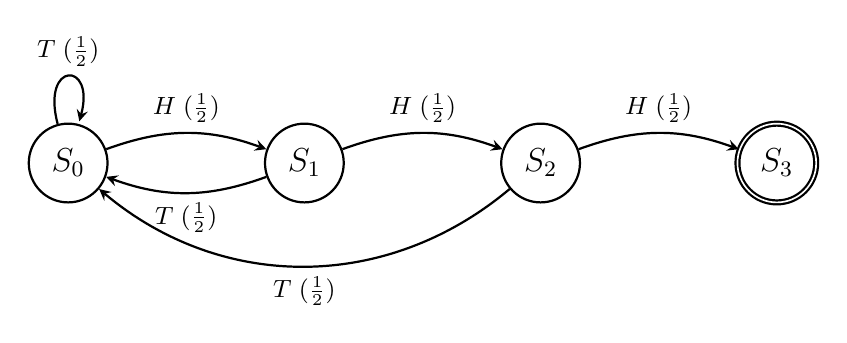
\begin{tikzpicture}[->, >=stealth, auto, node distance=3cm, thick,
    main node/.style={circle, draw, minimum size=1cm, font=\large}]

    \node[main node] (S0) {$S_0$};
    \node[main node] (S1) [right of=S0] {$S_1$};
    \node[main node] (S2) [right of=S1] {$S_2$};
    \node[main node, double] (S3) [right of=S2] {$S_3$};

    % Heads transitions (forward)
    \path[every node/.style={font=\small}]
        (S0) edge[bend left=20] node[above] {$H\;(\frac{1}{2})$} (S1)
        (S1) edge[bend left=20] node[above] {$H\;(\frac{1}{2})$} (S2)
        (S2) edge[bend left=20] node[above] {$H\;(\frac{1}{2})$} (S3);

    % Tails transitions (back to S0)
    \path[every node/.style={font=\small}]
        (S1) edge[bend left=20] node[below] {$T\;(\frac{1}{2})$} (S0)
        (S2) edge[bend left=40] node[below] {$T\;(\frac{1}{2})$} (S0);

    % Self-loop on S0
    \path[every node/.style={font=\small}]
        (S0) edge[loop above] node {$T\;(\frac{1}{2})$} (S0);

\end{tikzpicture}
\end{center}

\bigskip

\textbf{System of equations:}

Let $E_i$ be the expected number of tosses to reach $S_3$ starting from state $S_i$.

From each state, we toss the coin (cost 1). With probability $\frac{1}{2}$ we get heads (move forward), with probability $\frac{1}{2}$ we get tails (return to $S_0$):

\[
\begin{cases}
E_0 = 1 + \dfrac{1}{2}\,E_1 + \dfrac{1}{2}\,E_0 \\[10pt]
E_1 = 1 + \dfrac{1}{2}\,E_2 + \dfrac{1}{2}\,E_0 \\[10pt]
E_2 = 1 + \dfrac{1}{2}\cdot 0 + \dfrac{1}{2}\,E_0
\end{cases}
\]

\textbf{Solving:}

From the first equation:
\[
E_0 - \frac{1}{2}E_0 = 1 + \frac{1}{2}E_1 \implies \frac{1}{2}E_0 = 1 + \frac{1}{2}E_1 \implies E_0 = 2 + E_1
\]

From the third equation:
\[
E_2 = 1 + \frac{1}{2}E_0
\]

From the second equation:
\[
E_1 = 1 + \frac{1}{2}E_2 + \frac{1}{2}E_0 = 1 + \frac{1}{2}\left(1 + \frac{1}{2}E_0\right) + \frac{1}{2}E_0 = \frac{3}{2} + \frac{3}{4}E_0
\]

Substituting into $E_0 = 2 + E_1$:
\[
E_0 = 2 + \frac{3}{2} + \frac{3}{4}E_0 = \frac{7}{2} + \frac{3}{4}E_0
\]
\[
\frac{1}{4}E_0 = \frac{7}{2} \implies \boxed{E_0 = 14}
\]

\bigskip

The expected number of tosses to get three heads in a row is $\mathbf{14}$.


\section{Expected Tosses for $n$ Heads in a Row (Unfair Coin)}

\begin{exerciseBox}[Generalized Consecutive Heads]
For an unfair coin with probability $p$ of landing heads (and $q = 1-p$ for tails), what is the expected number of tosses to get $n$ consecutive heads in a row?
\end{exerciseBox}



\subsection*{Solution :}

We model this with a \textbf{Markov chain} with $n+1$ states based on the current streak of consecutive heads:

\begin{itemize}
    \item $S_0$: 0 consecutive heads (start or after a tail)
    \item $S_k$: $k$ consecutive heads, for $k = 1, \dots, n-1$
    \item $S_n$: $n$ consecutive heads (absorbing state -- goal reached)
\end{itemize}

\bigskip

\textbf{Markov Chain Graph:}

\begin{center}
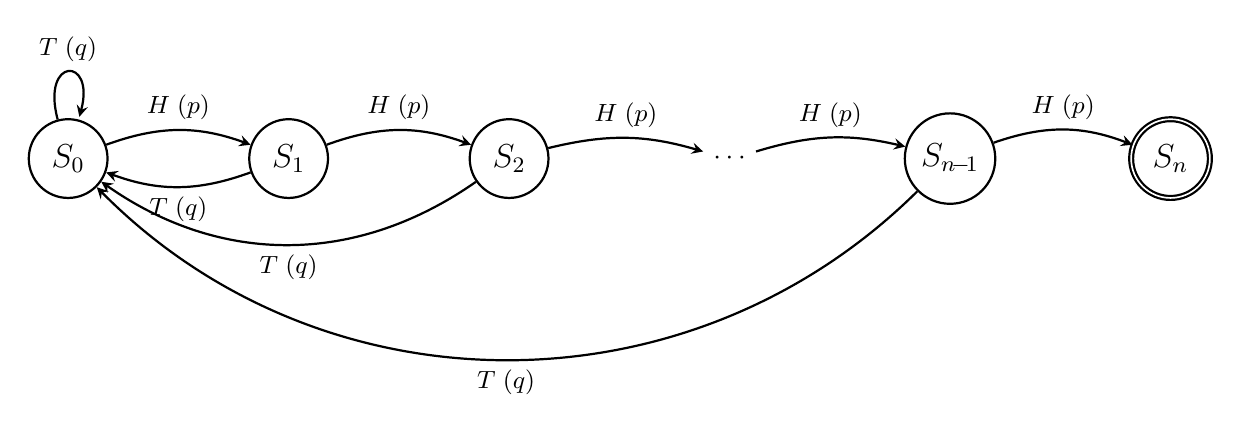
\begin{tikzpicture}[->, >=stealth, auto, node distance=2.8cm, thick,
    main node/.style={circle, draw, minimum size=1cm, font=\large}]

    \node[main node] (S0) {$S_0$};
    \node[main node] (S1) [right of=S0] {$S_1$};
    \node[main node] (S2) [right of=S1] {$S_2$};
    \node (dots) [right of=S2] {$\cdots$};
    \node[main node] (Sn1) [right of=dots] {$S_{n\!-\!1}$};
    \node[main node, double] (Sn) [right of=Sn1] {$S_n$};

    % Heads transitions (forward)
    \path[every node/.style={font=\small}]
        (S0) edge[bend left=20] node[above] {$H\;(p)$} (S1)
        (S1) edge[bend left=20] node[above] {$H\;(p)$} (S2)
        (S2) edge[bend left=15] node[above] {$H\;(p)$} (dots)
        (dots) edge[bend left=15] node[above] {$H\;(p)$} (Sn1)
        (Sn1) edge[bend left=20] node[above] {$H\;(p)$} (Sn);

    % Tails transitions (back to S0)
    \path[every node/.style={font=\small}]
        (S1) edge[bend left=20] node[below] {$T\;(q)$} (S0)
        (S2) edge[bend left=35] node[below] {$T\;(q)$} (S0)
        (Sn1) edge[bend left=45] node[below] {$T\;(q)$} (S0);

    % Self-loop on S0
    \path[every node/.style={font=\small}]
        (S0) edge[loop above] node {$T\;(q)$} (S0);

\end{tikzpicture}
\end{center}

\bigskip

\textbf{System of equations:}

Let $E_k$ be the expected number of tosses to reach $S_n$ from state $S_k$:

\[
\begin{cases}
E_0 = 1 + p\,E_1 + q\,E_0 \\[6pt]
E_k = 1 + p\,E_{k+1} + q\,E_0 \qquad \text{for } k = 1, \dots, n-2 \\[6pt]
E_{n-1} = 1 + p \cdot 0 + q\,E_0
\end{cases}
\]

\bigskip



The system of equations is:
\begin{align}
    E_0 &= 1 + p\,E_1 + q\,E_0 \label{eq:E0}\\
    E_k &= 1 + p\,E_{k+1} + q\,E_0 \quad \text{for } 1 \leq k \leq n-2 \label{eq:Ek}\\
    E_{n-1} &= 1 + q\,E_0 \label{eq:En1}\\
    E_n &= 0 \label{eq:En}
\end{align}

we now want to show taht : 
\[
    E_0 = \frac{1}{p} + \frac{1}{p^2} + \cdots + \frac{1}{p^n} = \sum_{k=1}^{n} \frac{1}{p^k}
\]


We define the successive differences:
\[
    d_k = E_k - E_{k+1}, \quad k = 0, 1, \ldots, n-1.
\]

\medskip
\textbf{Step 1: Simplify equation~\eqref{eq:E0}.}

From \textit{2.1}:
\[
    E_0 = 1 + p\,E_1 + q\,E_0
\]
Since $p + q = 1$, we have $E_0 - q\,E_0 = p\,E_0$, so:
\[
    p\,E_0 = 1 + p\,E_1 \implies E_0 - E_1 = \frac{1}{p}
\]
Therefore:
\[
    d_0 = \frac{1}{p}.
\]

\medskip
\textbf{Step 2: Derive a recurrence for $d_k$.}

From the general equation \textit{2.2}, for $1 \leq k \leq n-2$:
\[
    E_k = 1 + p\,E_{k+1} + (1 - p)\,E_0
\]
Expanding:
\[
    E_k = 1 + p\,E_{k+1} + E_0 - p\,E_0
\]
Rearranging:
\[
    E_k - p\,E_{k+1} = 1 + E_0 - p\,E_0
\]
Adding and subtracting $p\,E_k$ on the left-hand side:
\[
    p\,E_k + (1-p)\,E_k - p\,E_{k+1} = 1 + (1-p)\,E_0
\]
\[
    p(E_k - E_{k+1}) + (1-p)\,E_k = 1 + (1-p)\,E_0
\]
\[
    p(E_k - E_{k+1}) = 1 + (1-p)(E_0 - E_k)
\]
Using $q = 1-p$:
\begin{equation} \label{eq:recurrence}
    p\,d_k = 1 + q\,(E_0 - E_k)
\end{equation}


\medskip
\textbf{Step 3: Prove by induction that $d_k = \dfrac{1}{p^{k+1}}$.}

  
\textbf{Lemma : }

For all $0 \leq k \leq n-1$, we have $d_k = \dfrac{1}{p^{k+1}}$.

  

\textit{Base case} ($k = 0$): Already shown in Step~1: $d_0 = \dfrac{1}{p}$. \checkmark

\medskip
\textit{Inductive step:} Assume $d_j = \dfrac{1}{p^{j+1}}$ for all $0 \leq j \leq k-1$. We show $d_k = \dfrac{1}{p^{k+1}}$.

By telescoping:
\[
    E_0 - E_k = \sum_{j=0}^{k-1} d_j = \sum_{j=0}^{k-1} \frac{1}{p^{j+1}} = \frac{1}{p} + \frac{1}{p^2} + \cdots + \frac{1}{p^k}
\]

This is a geometric series with ratio $1/p$:
\[
    E_0 - E_k = \frac{1}{p} \cdot \frac{1 - (1/p)^k}{1 - 1/p} = \frac{1 - 1/p^k}{\displaystyle p - 1} = \frac{1 - 1/p^k}{-q} = \frac{1/p^k - 1}{q}
\]

Substituting into \eqref{eq:recurrence}:
\[
    p\,d_k = 1 + q \cdot \frac{1/p^k - 1}{q} = 1 + \frac{1}{p^k} - 1 = \frac{1}{p^k}
\]

Therefore:
\[
    d_k = \frac{1}{p^{k+1}}
\]

This completes the induction.

\medskip
\textbf{Step 4: Telescope to obtain $E_0$.}

Since $E_n = 0$:
\[
    E_0 = E_0 - E_n = \sum_{k=0}^{n-1} (E_k - E_{k+1}) = \sum_{k=0}^{n-1} d_k = \sum_{k=0}^{n-1} \frac{1}{p^{k+1}} = \sum_{k=1}^{n} \frac{1}{p^k}
\]

Therefore:
\[
    \boxed{\displaystyle E_0 = \frac{1}{p} + \frac{1}{p^2} + \cdots + \frac{1}{p^n}}
\]


\section{Le Problème du Collectionneur de Coupons}

\begin{exerciseBox}[Coupon Collector]
Il y a $N$ types de cartes différentes dans des paquets de céréales. Chaque paquet contient une carte choisie uniformément au hasard parmi les $N$ types. Combien de paquets faut-il acheter en moyenne pour obtenir la collection complète?
\end{exerciseBox}



\subsection*{Solution :}

Soit $T_i$ le nombre d'achats nécessaires pour trouver la $i$-ième nouvelle carte, sachant qu'on possède déjà $i-1$ cartes distinctes.

\bigskip

\textbf{Loi de $T_i$ :}

Lorsqu'on possède $i-1$ cartes, à chaque achat, la carte obtenue est nouvelle avec probabilité :
\[
p_i = \frac{N - (i-1)}{N}
\]
car il reste $N - (i-1)$ cartes qu'on n'a pas encore parmi les $N$ types. Chaque achat est indépendant, donc $T_i$ compte le nombre d'essais jusqu'au premier succès :

\[
\boxed{T_i \sim \mathrm{Geom}(p_i)} \qquad \text{avec} \quad p_i = \frac{N - (i-1)}{N}
\]

On a en particulier :
\[
\mathbb{E}[T_i] = \frac{1}{p_i} = \frac{N}{N - i + 1}
\]

\bigskip

\textbf{Nombre total de paquets :}

Le nombre total de paquets achetés pour compléter la collection est :
\[
T = T_1 + T_2 + \cdots + T_N
\]

Les $T_i$ sont indépendantes (chaque phase commence après la précédente). Par linéarité de l'espérance :

\[
\mathbb{E}[T] = \sum_{i=1}^{N} \mathbb{E}[T_i] = \sum_{i=1}^{N} \frac{N}{N - i + 1} = N \sum_{i=1}^{N} \frac{1}{i}
\]

\[
\boxed{\mathbb{E}[T] = N \cdot H_N = N \sum_{i=1}^{N} \frac{1}{i}}
\]

où $H_N = \displaystyle\sum_{i=1}^{N} \frac{1}{i}$ est le $N$-ième \textbf{nombre harmonique}.

\bigskip

\textbf{Équivalent asymptotique :}

En utilisant le développement classique $H_N = \ln(N) + \gamma + O\!\left(\frac{1}{N}\right)$, où $\gamma \approx 0.5772$ est la constante d'Euler--Mascheroni :

\[
\boxed{\mathbb{E}[T] \underset{N \to \infty}{\sim} N \ln(N)}
\]



\bigskip

\textbf{Variance :}

Les $T_i$ étant indépendantes, on a $\mathrm{Var}(T_i) = \dfrac{1-p_i}{p_i^2}$, d'où :
\[
\mathrm{Var}(T) = \sum_{i=1}^{N} \frac{1 - p_i}{p_i^2} = N^2 \sum_{i=1}^{N} \frac{1}{i^2} - N\sum_{i=1}^{N}\frac{1}{i}
\]

Asymptotiquement, comme $\displaystyle\sum_{i=1}^{N} \frac{1}{i^2} \to \frac{\pi^2}{6}$ :
\[
\mathrm{Var}(T) \underset{N \to \infty}{\sim} \frac{\pi^2}{6}\,N^2
\]


\section{Gambler's Ruin}

\begin{exerciseBox}[Gambler's Ruin]
You have 100€ and play a coin-toss game, betting 1€ each round. You stop when you reach 0€ or 200€.

\textbf{Q1.} What is the probability of finishing at 200€?

\textbf{Q2.} What if the coin is biased with $P(\text{Heads}) = p \neq 1/2$?

\textbf{Q3.} In the fair case ($p = 1/2$), what is the expected number of rounds before the game ends?
\end{exerciseBox}

\subsection*{Solution}

\subsubsection*{Q1. Fair coin ($p = 1/2$)}

\textbf{Modelling.} Let $X_k = X_0 + \sum_{i=1}^{k} \varepsilon_i$ where $\varepsilon_i = \pm 1$ with probability $1/2$. Since $E[\varepsilon_i] = 0$, the process $(X_k)_{k \geq 0}$ is a \textbf{martingale}.

\textbf{Stopping time.} Define $\tau = \inf\{n \in \mathbb{N} : X_n = 0 \text{ or } X_n = 200\}$.

\textbf{Optional Stopping Theorem.} Since $X_\tau$ is bounded ($0 \leq X_\tau \leq 200$) and $\tau < \infty$ a.s., we can apply the Optional Stopping Theorem:
\[
E[X_\tau] = E[X_0] = 100.
\]
Decomposing $E[X_\tau]$:
\[
E[X_\tau] = 0 \cdot P(X_\tau = 0) + 200 \cdot P(X_\tau = 200) = 100
\]
\[
\boxed{P(X_\tau = 200) = \frac{1}{2}}
\]

\subsubsection*{Q2. Biased coin ($p \neq 1/2$)}

When $p \neq 1/2$, $X_k$ is no longer a martingale since $E[X_{k+1} | X_k] = X_k + (p - q) \neq X_k$. We need to find a new martingale.

\textbf{Finding the right martingale.} We look for $f(x) = \lambda^x$ such that $(f(X_k))_k$ is a martingale. The condition $E[f(X_{k+1}) | X_k] = f(X_k)$ gives:

\[
E[f(X_{k+1}) | X_k] = f(X_k)
\]

\[
E[f(X_{k} + \epsilon_{k+1}) | X_k] = f(X_k)
\]

or : 
\[
E[f(X_{k} + \epsilon_{k+1}) | X_k] = pE[f(X_{k} + 1) | X_k] + qE[f(X_{k} - 1) | X_k]
\]

\[
E[f(X_{k} + \epsilon_{k+1}) | X_k] = pf(X_{k} + 1) + qf(X_{k} - 1)
\]


so that we have 

\[
pf(X_{k} + 1) + qf(X_{k} - 1)  = f(X_{k})
\]

\[
p \cdot \lambda^{X_k + 1} + q \cdot \lambda^{X_k - 1} = \lambda^{X_k}
\]

Dividing by $\lambda^{X_k}$:
\[
p\lambda + q\lambda^{-1} = 1 \implies p\lambda^2 - \lambda + q = 0
\]
The solutions are:
\[
\lambda = \frac{1 \pm \sqrt{1 - 4pq}}{2p} = \frac{1 \pm (p - q)}{2p}
\]
which gives $\lambda = 1$ (trivial) or $\lambda = q/p$. Therefore:
\[
M_k = \left(\frac{q}{p}\right)^{X_k} \text{ is a martingale.}
\]

\textbf{Applying the Optional Stopping Theorem to $M_k$:}
\[
E[M_\tau] = E[M_0] = \left(\frac{q}{p}\right)^{100}
\]
\[
\left(\frac{q}{p}\right)^{0} \cdot P(X_\tau = 0) + \left(\frac{q}{p}\right)^{200} \cdot P(X_\tau = 200) = \left(\frac{q}{p}\right)^{100}
\]
Using $P(X_\tau = 0) = 1 - P(X_\tau = 200)$ and solving:
\[
\boxed{P(X_\tau = 200) = \frac{(q/p)^{100} - 1}{(q/p)^{200} - 1}}
\]

% \textbf{Verification:} When $p = q = 1/2$, we have $q/p = 1$ and the formula is of the form $0/0$. Applying L'Hôpital's rule (setting $r = q/p \to 1$):
% \[
% \lim_{r \to 1} \frac{r^{100} - 1}{r^{200} - 1} = \lim_{r \to 1} \frac{100\, r^{99}}{200\, r^{199}} = \frac{100}{200} = \frac{1}{2} \quad \checkmark
% \]

\subsubsection*{Q3. Expected duration $E[\tau]$ in the fair case}

\textbf{Finding another martingale.} We claim that $M_k = X_k^2 - k$ is a martingale.

\textbf{Proof.} Since $X_{k+1} = X_k + \varepsilon_{k+1}$:
\[
X_{k+1}^2 = X_k^2 + 2X_k \varepsilon_{k+1} + \varepsilon_{k+1}^2
\]
Taking conditional expectations:
\[
E[X_{k+1}^2 \mid \mathcal{F}_k] = X_k^2 + 2X_k \underbrace{E[\varepsilon_{k+1}]}_{=\,0} + \underbrace{E[\varepsilon_{k+1}^2]}_{=\,1} = X_k^2 + 1
\]
Therefore:
\[
E[X_{k+1}^2 - (k+1) \mid \mathcal{F}_k] = X_k^2 + 1 - (k+1) = X_k^2 - k \quad \checkmark
\]

\textbf{Applying the Optional Stopping Theorem to $M_k = X_k^2 - k$:}
\[
E[X_\tau^2 - \tau] = E[X_0^2] = 100^2 = 10\,000
\]
Computing $E[X_\tau^2]$ using the result from Q1:
\[
E[X_\tau^2] = 0^2 \cdot \frac{1}{2} + 200^2 \cdot \frac{1}{2} = 20\,000
\]
Therefore:
\[
20\,000 - E[\tau] = 10\,000
\]
\[
\boxed{E[\tau] = 10\,000}
\]


\section{Le Bâton Cassé en Triangle}

\begin{exerciseBox}[Le Bâton Cassé]
On prend un bâton de longueur 1. On choisit deux points uniformément au hasard sur le bâton, ce qui le casse en trois morceaux. Quelle est la probabilité que les trois morceaux puissent former un triangle?
\end{exerciseBox}



\subsection*{Solution :}

\textbf{Partie 1 : Simplification de la condition.}

\bigskip

Notons $a$, $b$, $c$ les longueurs des trois morceaux. On forme un triangle si et seulement si l'inégalité triangulaire est vérifiée :
\[
P(\triangle) = P(a + b > c \;\cap\; a + c > b \;\cap\; b + c > a)
\]

Or $a + b + c = 1$, donc $a + b = 1 - c$. Ainsi $a + b > c \iff 1 - c > c \iff c < \frac{1}{2}$. De même pour les deux autres inégalités. D'où :

\[
\boxed{P(\triangle) = P\!\left(a < \frac{1}{2} \;\cap\; b < \frac{1}{2} \;\cap\; c < \frac{1}{2}\right)}
\]

\bigskip

\textbf{Partie 2 : Calcul de la probabilité.}

\bigskip

Soient $U \sim \mathcal{U}(0,1)$ et $V \sim \mathcal{U}(0,1)$ indépendantes les deux points de cassure. Le couple $(U,V)$ est uniforme sur le carré unité $[0,1]^2$. Les trois morceaux s'écrivent :
\[
a = \min(U,V), \qquad b = |V - U|, \qquad c = 1 - \max(U,V)
\]

\begin{center}
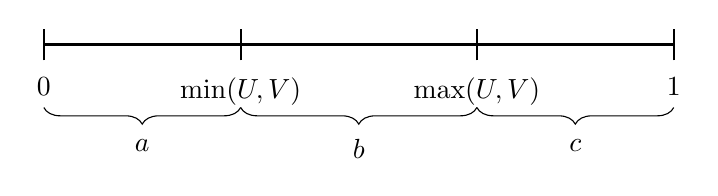
\begin{tikzpicture}
    \draw[thick] (0,0) -- (8,0);
    \draw[thick] (0,-0.2) -- (0,0.2);
    \draw[thick] (8,-0.2) -- (8,0.2);
    \draw[thick] (2.5,-0.2) -- (2.5,0.2);
    \draw[thick] (5.5,-0.2) -- (5.5,0.2);
    \node[below] at (0,-0.3) {$0$};
    \node[below] at (8,-0.3) {$1$};
    \node[below] at (2.5,-0.3) {$\min(U,V)$};
    \node[below] at (5.5,-0.3) {$\max(U,V)$};
    \draw[decorate, decoration={brace, amplitude=6pt, mirror}] (0,-0.8) -- (2.5,-0.8) node[midway, below=8pt] {$a$};
    \draw[decorate, decoration={brace, amplitude=6pt, mirror}] (2.5,-0.8) -- (5.5,-0.8) node[midway, below=8pt] {$b$};
    \draw[decorate, decoration={brace, amplitude=6pt, mirror}] (5.5,-0.8) -- (8,-0.8) node[midway, below=8pt] {$c$};
\end{tikzpicture}
\end{center}

\bigskip

Par la formule des probabilités totales :
\[
P(\triangle) = P(\triangle \mid U < V)\,P(U < V) + P(\triangle \mid V < U)\,P(V < U)
\]

Or $P(U < V) = P(V < U) = \dfrac{1}{2}$ (l'aire du triangle sous la diagonale vaut la moitié de l'aire du carré). De plus, par symétrie des rôles de $U$ et $V$ :
\[
P(\triangle \mid U < V) = P(\triangle \mid V < U)
\]

Donc :
\[
P(\triangle) = 2 \times \frac{1}{2} \times P(\triangle \mid U < V) = P(\triangle \mid U < V)
\]

\textbf{Sans perte de généralité}, on suppose $U < V$. Alors $a = U$, $b = V - U$, $c = 1 - V$, et :
\[
P(\triangle) = P\!\left(U < \frac{1}{2} \;\cap\; V - U < \frac{1}{2} \;\cap\; 1 - V < \frac{1}{2}\right) = P\!\left(U < \frac{1}{2} \;\cap\; V < U + \frac{1}{2} \;\cap\; V > \frac{1}{2}\right)
\]

\bigskip

On représente ces trois conditions dans le carré unité (sous la contrainte $U < V$) :

\begin{center}
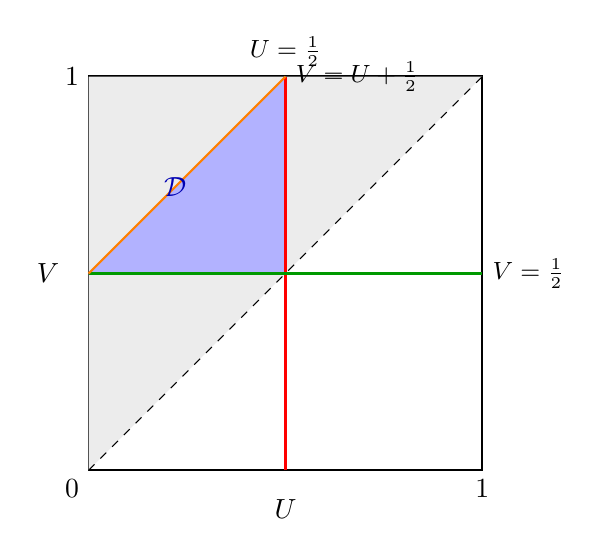
\begin{tikzpicture}[scale=5]
    % Carré unité
    \draw[thick] (0,0) rectangle (1,1);

    % Triangle U < V
    \fill[gray!15] (0,0) -- (1,1) -- (0,1) -- cycle;

    % Zone favorable (triangle)
    \fill[blue!30] (0,0.5) -- (0.5,0.5) -- (0.5,1) -- cycle;

    % Diagonale U = V
    \draw[dashed] (0,0) -- (1,1);
    % U = 1/2
    \draw[red, thick] (0.5,0) -- (0.5,1) node[above, black, font=\small] {$U = \frac{1}{2}$};
    % V = 1/2
    \draw[green!60!black, thick] (0,0.5) -- (1,0.5) node[right, black, font=\small] {$V = \frac{1}{2}$};
    % V = U + 1/2
    \draw[orange, thick] (0,0.5) -- (0.5,1) node[right, black, font=\small] {$V = U + \frac{1}{2}$};

    % Labels
    \node at (0.22,0.72) {\textcolor{blue!70!black}{\textbf{$\mathcal{D}$}}};

    % Axes
    \node[below] at (0.5,-0.05) {$U$};
    \node[left] at (-0.05,0.5) {$V$};
    \node[below left] at (0,0) {$0$};
    \node[below] at (1,0) {$1$};
    \node[left] at (0,1) {$1$};
\end{tikzpicture}
\end{center}

La zone favorable $\mathcal{D}$ est le triangle de sommets $\left(0,\frac{1}{2}\right)$, $\left(\frac{1}{2},\frac{1}{2}\right)$, $\left(\frac{1}{2},1\right)$, dont l'aire vaut :
\[
\mathcal{A}(\mathcal{D}) = \frac{1}{2} \times \frac{1}{2} \times \frac{1}{2} = \frac{1}{8}
\]

\begin{figure}[h]
    \centering
    \includegraphics[width=0.6\textwidth]{./images/desmos-graph.png}
    \caption{Fig of diff lines}
    \label{fig:desmos-img}
\end{figure}

Puisque $(U,V)$ est uniforme sur le carré d'aire 1 :
\[
P(\triangle \mid U < V) = \frac{\mathcal{A}(\mathcal{D})}{P(U<V)} = \frac{\frac{1}{8}}{\frac{1}{2}} = \frac{1}{4}
\]

Finalement :

\[
\boxed{P(\triangle) = \frac{1}{4}}
\]



\section{Le Paradoxe des Anniversaires}

\begin{exerciseBox}[Birthday Problem]
Dans une pièce, il y a $n$ personnes. On suppose que les anniversaires sont répartis uniformément sur les 365 jours de l'année (on ignore les années bissextiles), et que les anniversaires sont indépendants.

Quel est le nombre minimum de personnes $n$ pour que la probabilité qu'au moins deux personnes partagent le même anniversaire dépasse 50\%?
\end{exerciseBox}



\subsection*{Solution :}

\textbf{Passage au complémentaire :}

Notons $A$ l'événement « au moins deux personnes partagent le même anniversaire » et $J_i$ l'anniversaire de la personne $i$. On a :

\[
P(A) = 1 - P(\bar{A}) = 1 - P\!\left(\forall\, i \neq j,\; J_i \neq J_j\right)
\]

\bigskip

\textbf{Calcul de $P(\bar{A})$ :}

Notons $A_k$ l'événement « la $k$-ième personne a un anniversaire différent de toutes les précédentes ». Alors :

\[
P(\bar{A}) = P\!\left(\bigcap_{k=2}^{n} A_k\right)
\]

Par la formule des probabilités composées (chaîne) :

\[
P\!\left(\bigcap_{k=2}^{n} A_k\right) = \prod_{k=2}^{n} P\!\left(A_k \mid A_2 \cap A_3 \cap \cdots \cap A_{k-1}\right)
\]

Sachant que les $k-1$ premières personnes ont toutes des anniversaires distincts, la $k$-ième personne doit éviter $k-1$ jours parmi 365 :

\[
P\!\left(A_k \mid A_2 \cap \cdots \cap A_{k-1}\right) = \frac{365 - (k-1)}{365}
\]

D'où :

\[
P(\bar{A}) = \prod_{k=2}^{n} \frac{365 - (k-1)}{365} = \prod_{k=0}^{n-1} \left(1 - \frac{k}{365}\right)
\]

\bigskip

\textbf{Approximation :}

On utilise $\ln(1 - x) \approx -x$ pour $x$ petit :

\[
\ln P(\bar{A}) = \sum_{k=0}^{n-1} \ln\!\left(1 - \frac{k}{365}\right) \approx -\sum_{k=0}^{n-1} \frac{k}{365} = -\frac{n(n-1)}{2 \times 365}
\]

Donc :
\[
P(\bar{A}) \approx e^{-\frac{n(n-1)}{730}}
\]

On cherche $n$ tel que $P(A) > \frac{1}{2}$, soit $P(\bar{A}) < \frac{1}{2}$ :

\[
e^{-\frac{n(n-1)}{730}} < \frac{1}{2} \implies \frac{n(n-1)}{730} > \ln 2 \implies n(n-1) > 730 \ln 2 \approx 505.97
\]

En approximant $n(n-1) \approx n^2$ :
\[
n > \sqrt{730 \ln 2} \approx 22.49
\]

Donc $n \geq 23$.

% \bigskip

% \textbf{Vérification par calcul exact :}

% \[
% P(\bar{A})\big|_{n=22} = \prod_{k=0}^{21}\left(1 - \frac{k}{365}\right) \approx 0.5243 \implies P(A)\big|_{n=22} \approx 0.4757 < 0.5
% \]

% \[
% P(\bar{A})\big|_{n=23} = \prod_{k=0}^{22}\left(1 - \frac{k}{365}\right) \approx 0.4927 \implies P(A)\big|_{n=23} \approx 0.5073 > 0.5
% \]

\bigskip

\[
\boxed{n = 23}
\]

Il suffit de 23 personnes pour que la probabilité qu'au moins deux partagent le même anniversaire dépasse 50\%. Ce résultat, souvent contre-intuitif, est connu sous le nom de \textbf{paradoxe des anniversaires}.



\section{Voir Toutes les Faces d'un Dé}

\begin{exerciseBox}[Toutes les Faces du Dé]
On lance un dé équilibré à 6 faces, encore et encore, jusqu'à avoir obtenu chaque face au moins une fois.

En moyenne, combien de lancers faut-il pour voir les 6 faces?
\end{exerciseBox}



\subsection*{Solution :}

C'est une application directe du \textbf{problème du collectionneur de coupons} avec $N = 6$.

\bigskip

\textbf{Découpage en phases :}

Soit $T_i$ le nombre de lancers nécessaires pour obtenir la $i$-ième nouvelle face, sachant qu'on possède déjà $i-1$ faces distinctes.

À chaque lancer, la probabilité d'obtenir une face nouvelle est :
\[
p_i = \frac{6 - (i-1)}{6} = \frac{7 - i}{6}
\]

Chaque lancer étant indépendant, $T_i$ compte le nombre d'essais jusqu'au premier succès, donc :
\[
T_i \sim \mathrm{Geom}(p_i) \qquad \text{avec} \quad \mathbb{E}[T_i] = \frac{1}{p_i} = \frac{6}{7-i}
\]

\bigskip

\textbf{Détail de chaque phase :}

\begin{center}
\renewcommand{\arraystretch}{1.5}
\begin{tabular}{c|c|c|c}
Phase $i$ & Faces déjà vues & $p_i$ & $\mathbb{E}[T_i]$ \\
\hline
1 & 0 & $\frac{6}{6} = 1$ & $1$ \\
2 & 1 & $\frac{5}{6}$ & $\frac{6}{5}$ \\
3 & 2 & $\frac{4}{6}$ & $\frac{6}{4}$ \\
4 & 3 & $\frac{3}{6}$ & $\frac{6}{3}$ \\
5 & 4 & $\frac{2}{6}$ & $\frac{6}{2}$ \\
6 & 5 & $\frac{1}{6}$ & $\frac{6}{1}$ \\
\end{tabular}
\end{center}

\bigskip

\textbf{Nombre total de lancers :}

Le nombre total est $T = T_1 + T_2 + \cdots + T_6$. Les $T_i$ étant indépendantes, par linéarité de l'espérance :

\[
\mathbb{E}[T] = \sum_{i=1}^{6} \mathbb{E}[T_i] = \sum_{i=1}^{6} \frac{6}{7-i} = 6\sum_{k=1}^{6} \frac{1}{k} = 6\left(1 + \frac{1}{2} + \frac{1}{3} + \frac{1}{4} + \frac{1}{5} + \frac{1}{6}\right)
\]

\[
\mathbb{E}[T] = 6 \times \frac{49}{20} = \frac{294}{20} = \frac{147}{10}
\]

\[
\boxed{\mathbb{E}[T] = 14.7 \text{ lancers}}
\]

\section{Fair coin from biased coin (Von Neumann)}

\begin{exerciseBox}[Générer une pièce équitable à partir d'une pièce biaisée (Von Neumann)]
Tu as une pièce biaisée :
\[
\mathbb{P}(H)=p,\qquad 0<p<1,
\]
où $p$ est inconnu.

Tu veux générer un tirage pile/face \textbf{équitable} (probabilité $1/2$) en utilisant uniquement cette pièce, sans connaître $p$.

\textbf{Question :} quelle procédure utilises-tu ? Montrer que la sortie est équitable.
\end{exerciseBox}

\subsection*{Solution :}

\paragraph{Procédure (algorithme de Von Neumann)}
On répète l'expérience suivante :
\begin{itemize}
\item Lancer la pièce \textbf{deux fois}.
\item Si on obtient $HH$ ou $TT$, on \textbf{rejette} et on recommence.
\item Si on obtient $HT$, on \textbf{sort} $H$.
\item Si on obtient $TH$, on \textbf{sort} $T$.
\end{itemize}

\subsubsection*{Méthode 1 — Intuition (conditionnement, sans preuve lourde)}

Considérons un essai \emph{accepté}, c'est-à-dire l'événement
\[
A=\{HT\ \text{ou}\ TH\}.
\]
On a :
\[
\mathbb{P}(HT)=p(1-p),\qquad \mathbb{P}(TH)=(1-p)p=p(1-p).
\]
Donc :
\[
\mathbb{P}(HT\mid A)=\frac{\mathbb{P}(HT)}{\mathbb{P}(HT)+\mathbb{P}(TH)}
=\frac{p(1-p)}{2p(1-p)}=\frac12.
\]
Ainsi, conditionnellement au fait qu'on accepte, $HT$ et $TH$ sont équiprobables, donc la sortie est équitable.

\[
\boxed{\mathbb{P}(Y=H)=\frac12 \quad\text{et}\quad \mathbb{P}(Y=T)=\frac12.}
\]

\subsubsection*{Méthode 2 — Preuve rigoureuse (via le premier essai accepté)}

\paragraph{Définition rigoureuse}

On fait des essais $k=1,2,3,\dots$.  
À l'essai $k$, on lance deux fois :
\[
(X_{k,1},X_{k,2})\in\{H,T\}^2.
\]

On note l'événement d'acceptation :
\[
A_k=\{(X_{k,1},X_{k,2})\in\{HT,TH\}\}.
\]
Alors
\[
\mathbb{P}(A_k)=\mathbb{P}(HT)+\mathbb{P}(TH)=p(1-p)+(1-p)p=2p(1-p).
\]

On définit le premier essai accepté :
\[
N=\min\{k\ge 1:\ A_k\ \text{se produit}\}.
\]

Puis on définit la variable de sortie :
\[
Y=
\begin{cases}
H & \text{si } (X_{N,1},X_{N,2})=HT,\\
T & \text{si } (X_{N,1},X_{N,2})=TH.
\end{cases}
\]

\paragraph{Objectif}
Montrer :
\[
\mathbb{P}(Y=H)=\frac12.
\]

\paragraph{Étape 1 — Décomposition selon $N$}

\[
\mathbb{P}(Y=H)=\sum_{n\ge 1}\mathbb{P}(Y=H,\ N=n).
\]

Or :
\[
\{Y=H,\ N=n\}
=
\big(A_1^c\cap\cdots\cap A_{n-1}^c\big)\ \cap\ \{(X_{n,1},X_{n,2})=HT\}.
\]

Par indépendance entre essais :
\[
\mathbb{P}(Y=H,\ N=n)=\mathbb{P}(A_1^c\cap\cdots\cap A_{n-1}^c)\cdot \mathbb{P}((X_{n,1},X_{n,2})=HT).
\]

\paragraph{Étape 2 — Calcul des facteurs}

\[
\mathbb{P}((X_{n,1},X_{n,2})=HT)=p(1-p).
\]
De plus :
\[
\mathbb{P}(A_k^c)=1-\mathbb{P}(A_k)=1-2p(1-p),
\]
donc
\[
\mathbb{P}(A_1^c\cap\cdots\cap A_{n-1}^c)=\big(1-2p(1-p)\big)^{n-1}.
\]

Ainsi :
\[
\mathbb{P}(Y=H,\ N=n)=\big(1-2p(1-p)\big)^{n-1}\,p(1-p).
\]

\paragraph{Étape 3 — Somme géométrique}

\[
\mathbb{P}(Y=H)=\sum_{n\ge 1}\big(1-2p(1-p)\big)^{n-1}\,p(1-p).
\]
C'est une série géométrique avec $r=1-2p(1-p)$, donc
\[
\sum_{n\ge 1} r^{n-1}=\frac{1}{1-r}.
\]
Donc :
\[
\mathbb{P}(Y=H)
=
p(1-p)\cdot\frac{1}{1-(1-2p(1-p))}
=
p(1-p)\cdot\frac{1}{2p(1-p)}
=\frac12.
\]

\[
\boxed{\mathbb{P}(Y=H)=\frac12,\qquad \mathbb{P}(Y=T)=\frac12.}
\]


\section{Paradoxe de Saint-Pétersbourg}

\begin{exerciseBox}[Jeu de Saint-Pétersbourg]
On lance une pièce équilibrée répétitivement jusqu'à obtenir \emph{Face} pour la première fois.
Si Face apparaît au lancer numéro $n$, tu gagnes $2^n$ euros.

Combien es-tu prêt à payer pour jouer à ce jeu ?
\end{exerciseBox}

\subsection*{Solution :}

\subsubsection*{Partie 1 — Critère espérance (gain moyen)}

On note $(X_k)_{k\ge 1}$ la suite des résultats, où $X_k\in\{\text{Pile},\text{Face}\}$.

On définit le temps d'arrêt :
\[
N=\inf\{k\ge 1:\ X_k=\text{Face}\}.
\]
Le gain est alors
\[
G=2^N.
\]

Comme la pièce est équilibrée, $N$ suit une loi géométrique de paramètre $1/2$ :
\[
\mathbb{P}(N=n)=\Big(\frac12\Big)^n,\qquad n\ge 1.
\]

On calcule l'espérance :
\[
\mathbb{E}[G]
=\sum_{n=1}^{\infty}\mathbb{E}(2^N\mid N=n)\,\mathbb{P}(N=n)
=\sum_{n=1}^{\infty}2^n\cdot \Big(\frac12\Big)^n
=\sum_{n=1}^{\infty}1
=+\infty.
\]

Donc l'espérance du gain est infinie :
\[
\boxed{\mathbb{E}[G]=+\infty.}
\]
Avec le critère \og prix juste = espérance \fg, on obtiendrait donc un prix infini, ce qui est irréaliste en pratique.

\subsubsection*{Partie 2 — Critère utilité (aversion au risque) : $U(x)=\ln(x)$}

L'idée est que l'espérance $\mathbb{E}[G]$ n'est pas forcément un bon critère si on est averse au risque.
On regarde plutôt l'espérance d'utilité :
\[
\mathbb{E}[U(G)] = \mathbb{E}[\ln(G)].
\]

Or $\ln(G)=\ln(2^N)=N\ln(2)$, donc :
\[
\mathbb{E}[\ln(G)]
=\sum_{n=1}^{\infty}\mathbb{P}(N=n)\,\ln(2^n)
=\sum_{n=1}^{\infty}\Big(\frac12\Big)^n\, n\ln(2)
=\ln(2)\sum_{n=1}^{\infty}\frac{n}{2^n}.
\]

On calcule la série classique. Pour $|x|<1$ :
\[
\sum_{n=0}^{\infty}x^n=\frac{1}{1-x}.
\]
En dérivant :
\[
\sum_{n=1}^{\infty}n x^{n-1}=\frac{1}{(1-x)^2},
\]
puis en multipliant par $x$ :
\[
\sum_{n=1}^{\infty}n x^{n}=\frac{x}{(1-x)^2}.
\]
En prenant $x=\frac12$ :
\[
\sum_{n=1}^{\infty}\frac{n}{2^n}
=\frac{\frac12}{(1-\frac12)^2}
=\frac{\frac12}{(\frac12)^2}
=\frac{\frac12}{\frac14}=2.
\]

Donc :
\[
\mathbb{E}[\ln(G)] = \ln(2)\cdot 2 = 2\ln(2).
\]

\paragraph{Prix \og fair \fg\ sous utilité log}
On cherche $X$ tel que l'utilité certaine $\ln(X)$ égale l'utilité espérée :
\[
\ln(X)=\mathbb{E}[\ln(G)]=2\ln(2).
\]
Ainsi :
\[
X=e^{2\ln(2)}=e^{\ln(4)}=4.
\]

\[
\boxed{X=4\text{ euros}.}
\]

\paragraph{Conclusion}
\begin{itemize}
\item Le critère espérance donne un gain moyen infini, donc un prix infini (paradoxe).
\item Avec une utilité logarithmique (aversion au risque), un prix raisonnable est
\[
\boxed{4\text{ euros}.}
\]
\end{itemize}

\section{House Selling Problem}

\begin{exerciseBox}[Vendre sa maison avec coût d'attente]
Tu veux vendre ta maison. Chaque jour, un acheteur potentiel arrive et te propose un prix. Les offres $(X_n)_{n\ge1}$ sont i.i.d. et uniformes sur $[0,1]$ (en millions d'euros).

Chaque jour, tu dois immédiatement décider :
\begin{itemize}
\item \textbf{Accepter} l'offre $\Rightarrow$ la maison est vendue, le jeu s'arrête.
\item \textbf{Refuser} $\Rightarrow$ l'acheteur part et ne revient jamais.
\end{itemize}

Il y a un coût d'attente : chaque jour supplémentaire te coûte $c$ (en millions d'euros).

\textbf{Q1.} Quelle est la stratégie optimale ? Quel est le gain maximal espéré $V^*$ et le temps d'attente moyen ?
\end{exerciseBox}

\subsection*{Solution :}

\subsubsection*{1) Stratégie à seuil et équation de Bellman}

On suppose une stratégie à seuil $s\in[0,1]$ :
\[
\text{Accepter si } X\ge s,\qquad \text{Refuser si } X<s.
\]

Notons $V$ la valeur espérée du jeu (gain net maximal) en début de journée.

À chaque jour :
\begin{itemize}
\item avec probabilité $\mathbb{P}(X\ge s)=1-s$, on accepte et on reçoit en moyenne
$\mathbb{E}[X\mid X\ge s]$ ;
\item avec probabilité $\mathbb{P}(X<s)=s$, on refuse, on paie le coût $c$, et on se retrouve
dans le \emph{même} problème (valeur $V$).
\end{itemize}

Donc l'équation de Bellman est :
\[
V=(1-s)\,\mathbb{E}[X\mid X\ge s]+s\,(V-c).
\]

\subsubsection*{2) Calcul de $\mathbb{E}[X\mid X\ge s]$ (uniforme)}

Si $X\sim \mathcal{U}[0,1]$, alors conditionnellement à $\{X\ge s\}$, on a $X\sim \mathcal{U}[s,1]$,
donc :
\[
\mathbb{E}[X\mid X\ge s]=\frac{s+1}{2}.
\]

On remplace dans Bellman :
\[
V=(1-s)\frac{1+s}{2}+s(V-c).
\]
Donc :
\[
V=\frac{1-s^2}{2}+sV-sc
\quad\Longrightarrow\quad
V(1-s)=\frac{1-s^2}{2}-sc.
\]
Comme $1-s>0$ (si $s<1$), on obtient :
\[
V(s)=\frac{1-s^2}{2(1-s)}-\frac{sc}{1-s}
=\frac{1+s}{2}-\frac{sc}{1-s}.
\]

\subsubsection*{3) Optimisation en $s$}

On dérive :
\[
V'(s)=\frac12-\frac{c}{(1-s)^2}.
\]
Condition du maximum :
\[
V'(s)=0
\quad\Longleftrightarrow\quad
\frac12=\frac{c}{(1-s)^2}
\quad\Longleftrightarrow\quad
(1-s)^2=2c.
\]
Ainsi (solution dans $[0,1]$) :
\[
\boxed{s^*=1-\sqrt{2c}}.
\]

\paragraph{Condition de validité}
On doit avoir $s^*\ge 0$, donc
\[
1-\sqrt{2c}\ge 0
\quad\Longleftrightarrow\quad
c\le \frac12.
\]
Si $c>\frac12$, le coût d'attente est trop élevé et il est optimal d'accepter immédiatement (seuil $0$).

\subsubsection*{4) Valeur optimale $V^*$}

Pour $c\le \frac12$, on calcule :
\[
V^*=V(s^*)=\frac{1+s^*}{2}-\frac{s^*c}{1-s^*}.
\]
Avec $1-s^*=\sqrt{2c}$ et $s^*=1-\sqrt{2c}$, on obtient :
\[
\boxed{V^*=1-\sqrt{2c}+c}.
\]
On remarque aussi la relation classique :
\[
\boxed{s^*=V^*-c}.
\]

Pour $c>\frac12$ (seuil $s^*=0$), on accepte la première offre :
\[
V^*=\mathbb{E}[X]=\frac12.
\]

\subsubsection*{5) Temps d'attente moyen}

Soit $\tau$ le jour de vente (premier jour où $X_\tau\ge s^*$).
Alors $\tau$ suit une loi géométrique de paramètre
\[
\mathbb{P}(X\ge s^*)=1-s^*.
\]
Donc :
\[
\mathbb{E}[\tau]=\frac{1}{1-s^*}.
\]

Pour $c\le \frac12$, $1-s^*=\sqrt{2c}$, donc :
\[
\boxed{\mathbb{E}[\tau]=\frac{1}{\sqrt{2c}}.}
\]

Pour $c>\frac12$, $s^*=0$ donc $\mathbb{E}[\tau]=1$ (vente immédiate en moyenne).

\subsubsection*{Résumé}

\[
\boxed{
s^*=
\begin{cases}
1-\sqrt{2c} & \text{si } c\le \frac12,\\
0 & \text{si } c>\frac12,
\end{cases}
\qquad
V^*=
\begin{cases}
1-\sqrt{2c}+c & \text{si } c\le \frac12,\\
\frac12 & \text{si } c>\frac12,
\end{cases}
\qquad
\mathbb{E}[\tau]=
\begin{cases}
\frac{1}{\sqrt{2c}} & \text{si } c\le \frac12,\\
1 & \text{si } c>\frac12.
\end{cases}
}
\]

\section{Drunk Man on a Cliff}

\begin{exerciseBox}[Homme ivre au bord d'une falaise]
Un homme ivre se trouve à $1$ pas du bord d'une falaise. À chaque instant, il fait un pas :
\begin{itemize}
\item vers la falaise (un pas en avant) avec probabilité $1/2$ ;
\item loin de la falaise (un pas en arrière) avec probabilité $1/2$.
\end{itemize}

On modélise sa distance au bord par un processus $(X_n)_{n\ge 0}$ à valeurs dans $\{0,1,2,\dots\}$, avec $X_0=1$ et $0$ est l'état \og chute \fg.

\textbf{Question 1 :} Quelle est la probabilité qu'il tombe de la falaise ?\\
\textbf{Question 2 :} En moyenne, combien de pas fait-il avant de tomber (sachant qu'il tombe) ?
\end{exerciseBox}

\subsection*{Solution :}

\subsubsection*{Setup}

On pose
\[
X_n = 1 + \sum_{k=1}^{n}\varepsilon_k,
\qquad \text{où } \varepsilon_k\in\{-1,+1\},\ \mathbb{P}(\varepsilon_k=1)=\mathbb{P}(\varepsilon_k=-1)=\frac12.
\]
Le temps de chute est
\[
\tau=\inf\{n\ge 1:\ X_n=0\}.
\]

\subsubsection*{Question 1 : Calcul de $\mathbb{P}(\tau<\infty)$}

Notons
\[
p=\mathbb{P}(\tau<\infty\mid X_0=1).
\]
Au premier pas :
\begin{itemize}
\item avec probabilité $1/2$, on va en $0$ et on tombe immédiatement ;
\item avec probabilité $1/2$, on va en $2$ et il faut tomber en partant de $2$.
\end{itemize}
Donc :
\[
p=\frac12+\frac12\,\mathbb{P}(\tau<\infty\mid X_0=2).
\]

\paragraph{Lien entre les probabilités depuis 1 et depuis 2}
Pour tomber en partant de $2$, il faut d'abord atteindre $1$, puis atteindre $0$ depuis $1$.
Par translation, la probabilité d'atteindre $1$ depuis $2$ est égale à la probabilité d'atteindre $0$ depuis $1$, donc elle vaut $p$.
Par la propriété de Markov forte, une fois arrivé en $1$, la probabilité de tomber ensuite est encore $p$, indépendamment du passé.
Ainsi :
\[
\mathbb{P}(\tau<\infty\mid X_0=2)=p\cdot p=p^2.
\]

On obtient donc l'équation :
\[
p=\frac12+\frac12 p^2.
\]
D'où :
\[
2p=1+p^2
\quad\Longleftrightarrow\quad
p^2-2p+1=0
\quad\Longleftrightarrow\quad
(p-1)^2=0.
\]
Donc :
\[
\boxed{p=1.}
\]
L'homme tombe avec certitude.

\subsubsection*{Question 2 : Temps moyen avant de tomber}

Comme $p=1$, \og sachant qu'il tombe \fg\ ne change rien :
\[
\mathbb{E}[\tau\mid \tau<\infty]=\mathbb{E}[\tau].
\]

Posons
\[
m=\mathbb{E}[\tau\mid X_0=1].
\]
Au premier pas :
\begin{itemize}
\item avec probabilité $1/2$, on tombe en $1$ pas ;
\item avec probabilité $1/2$, on va en $2$, et il faut ensuite tomber depuis $2$.
\end{itemize}

Par translation et la propriété de Markov forte, le temps moyen pour tomber depuis $2$ est la somme :
\[
\mathbb{E}[\tau\mid X_0=2] = \underbrace{\mathbb{E}[\text{temps pour aller de }2\text{ à }1]}_{=m}
+\underbrace{\mathbb{E}[\text{temps pour aller de }1\text{ à }0]}_{=m}
=2m.
\]

En comptant le premier pas, on a :
\[
m=\frac12\cdot 1+\frac12\cdot (1+2m).
\]
Développons :
\[
m=\frac12+\frac12+m
\quad\Longrightarrow\quad
m=1+m
\quad\Longrightarrow\quad
0=1,
\]
contradiction.

Donc l'hypothèse $m<\infty$ est fausse, et :
\[
\boxed{\mathbb{E}[\tau]=+\infty.}
\]

\subsubsection*{Conclusion}

\[
\boxed{\mathbb{P}(\text{tomber})=1 \quad\text{et}\quad \mathbb{E}[\tau]=+\infty.}
\]

C'est un exemple classique d'un temps d'arrêt $\tau$ presque sûrement fini, mais d'espérance infinie.

